% !TEX root = ../../main.tex

\subsection{Characterisation of trends}\label{def:trends}

The graphs in \autoref{def:fgr:tga-defects} summarize the 
trends in missing linker defects as calculated through 
the TGA plateau at \SI{420}{\degreeCelsius}. The DMF leached samples,
due to the multiple datapoints with different acid concentrations
show the clearest influence of this variable on defect
generation. Even small amounts of modulator leads to the decrease of 
the linker-to-node ratio, but the increase in concentration stops 
having an effect at around 20:1 equivalents. It is likely that
the trends are similar with other solvents, even if less 
datapoints are available.

\begin{figure}[htb]
    \centering

    \begin{subfigure}{0.25\linewidth}
        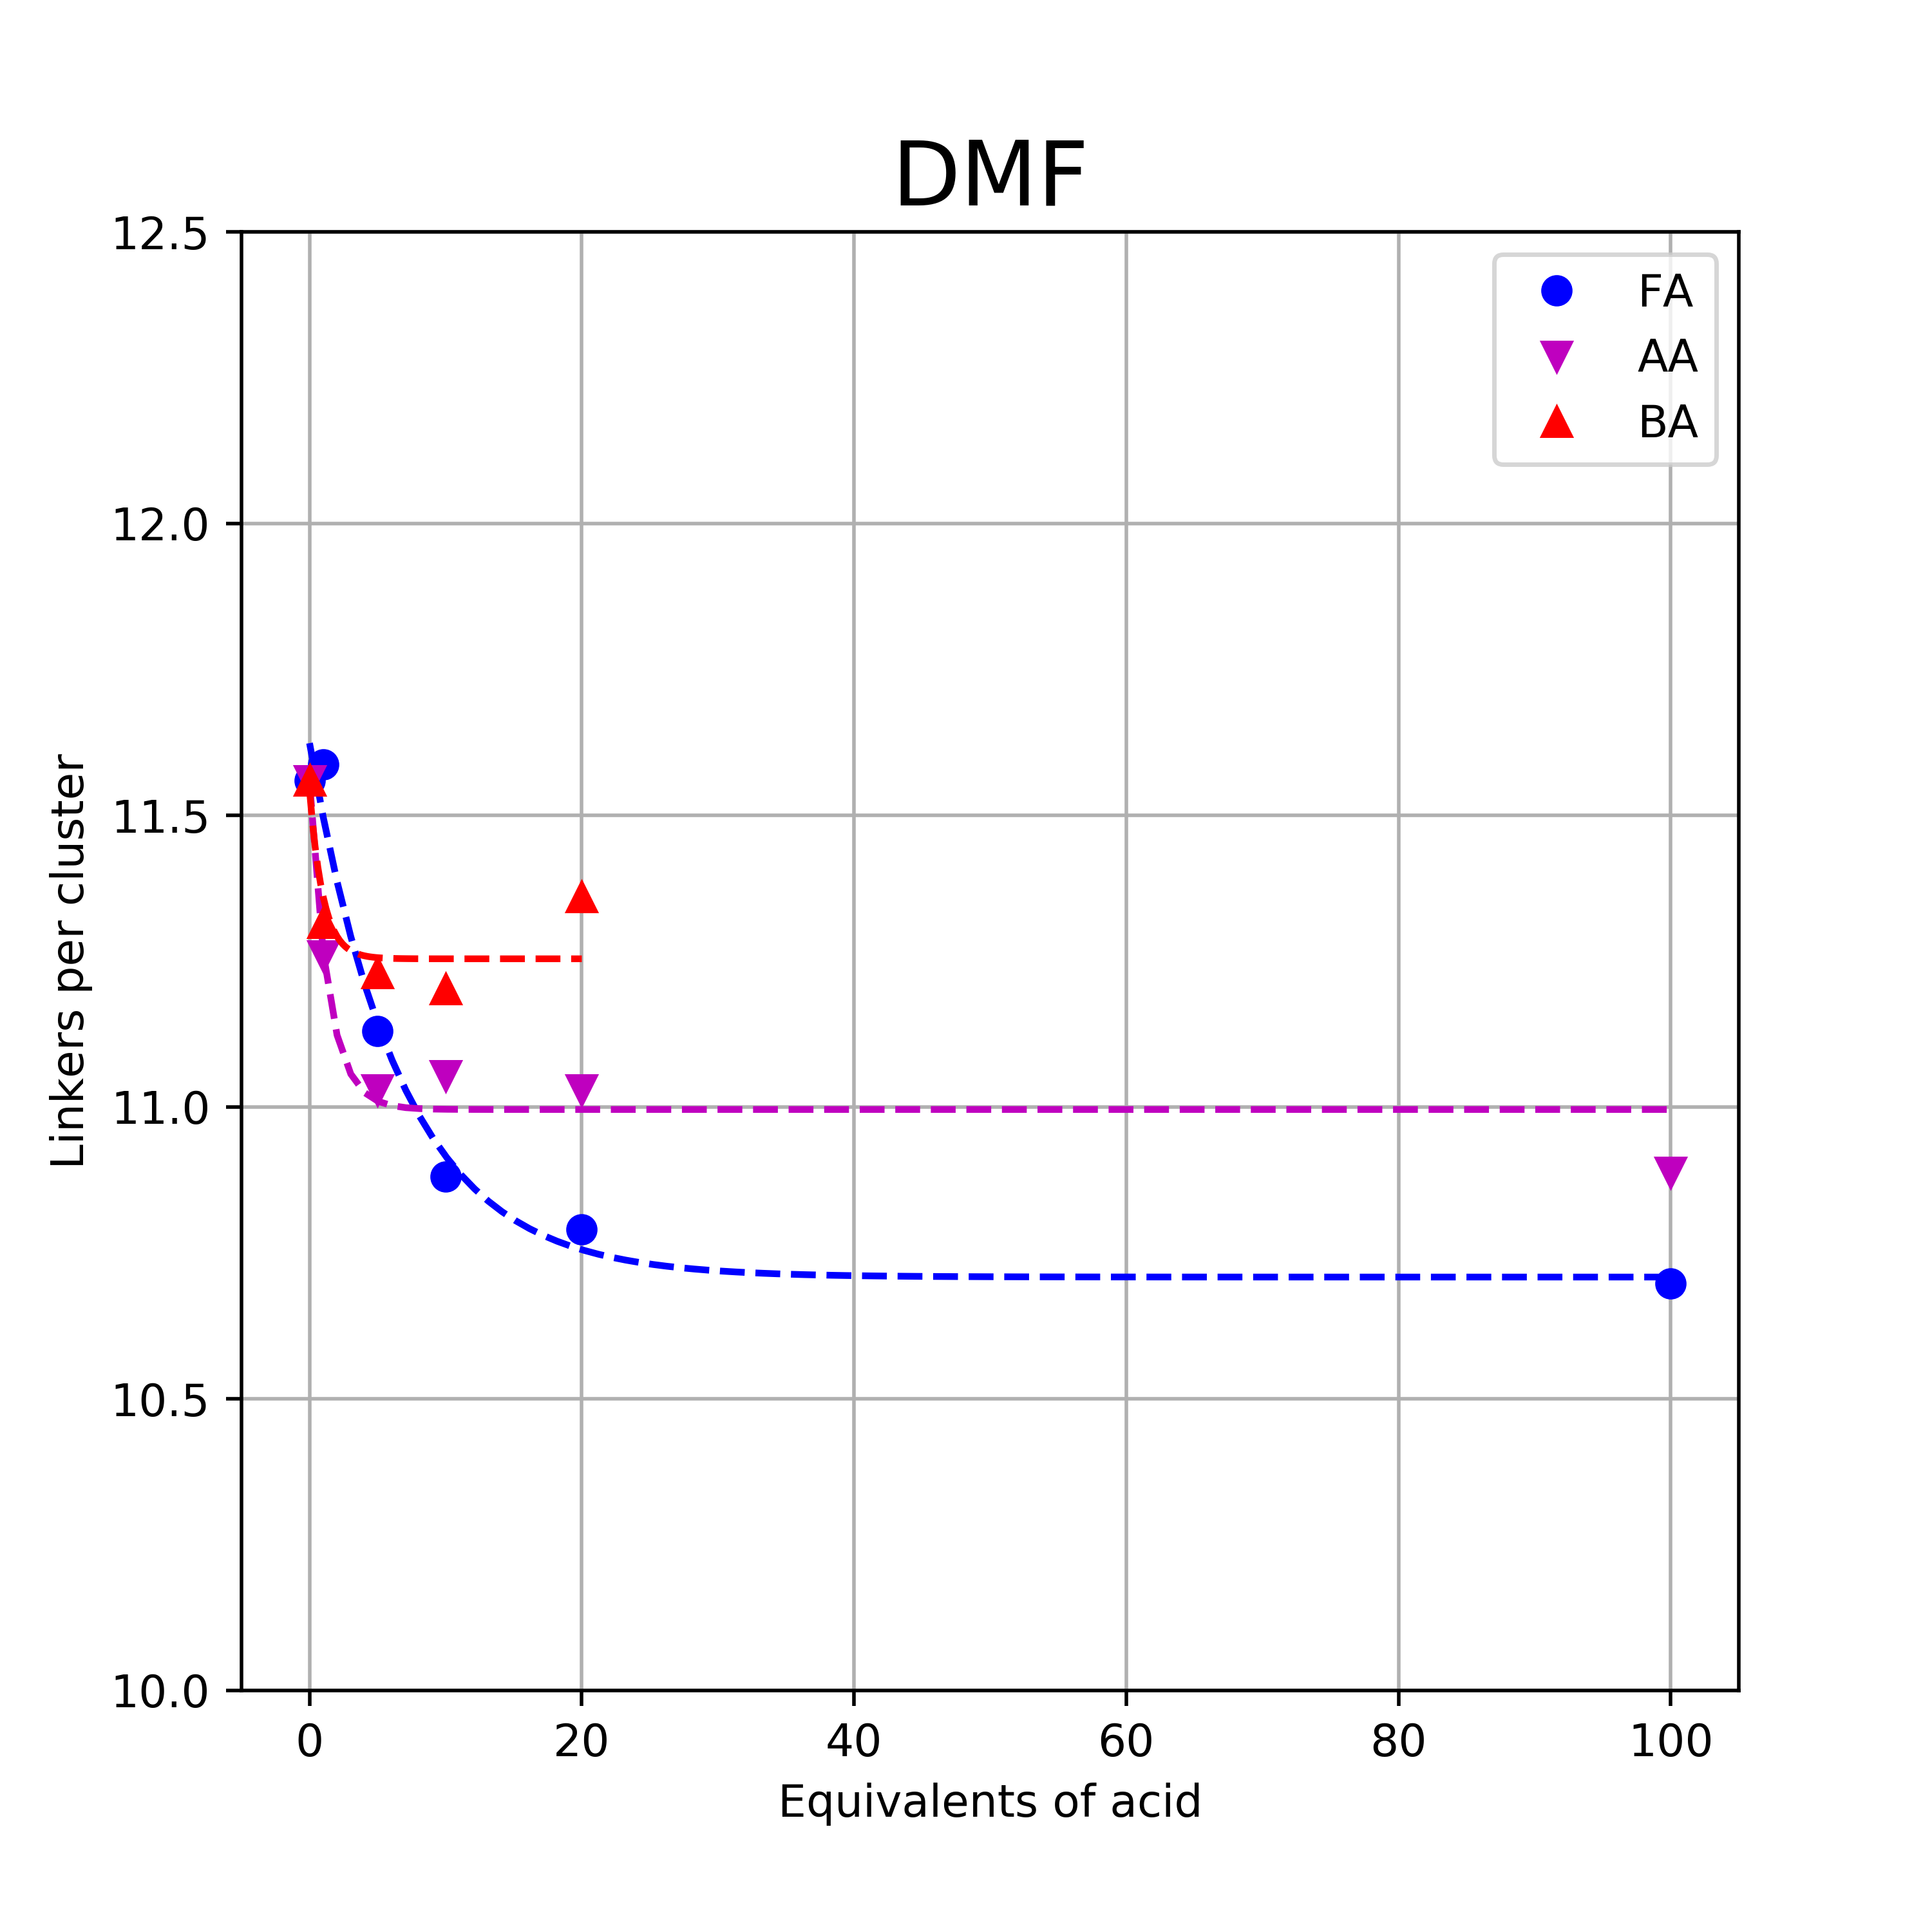
\includegraphics[width=\textwidth]{tga/DMF-def-overview}%
        \caption{}%
        \label{def:fgr:tga-dmf-linkers}
    \end{subfigure}%
    \begin{subfigure}{0.25\linewidth}
        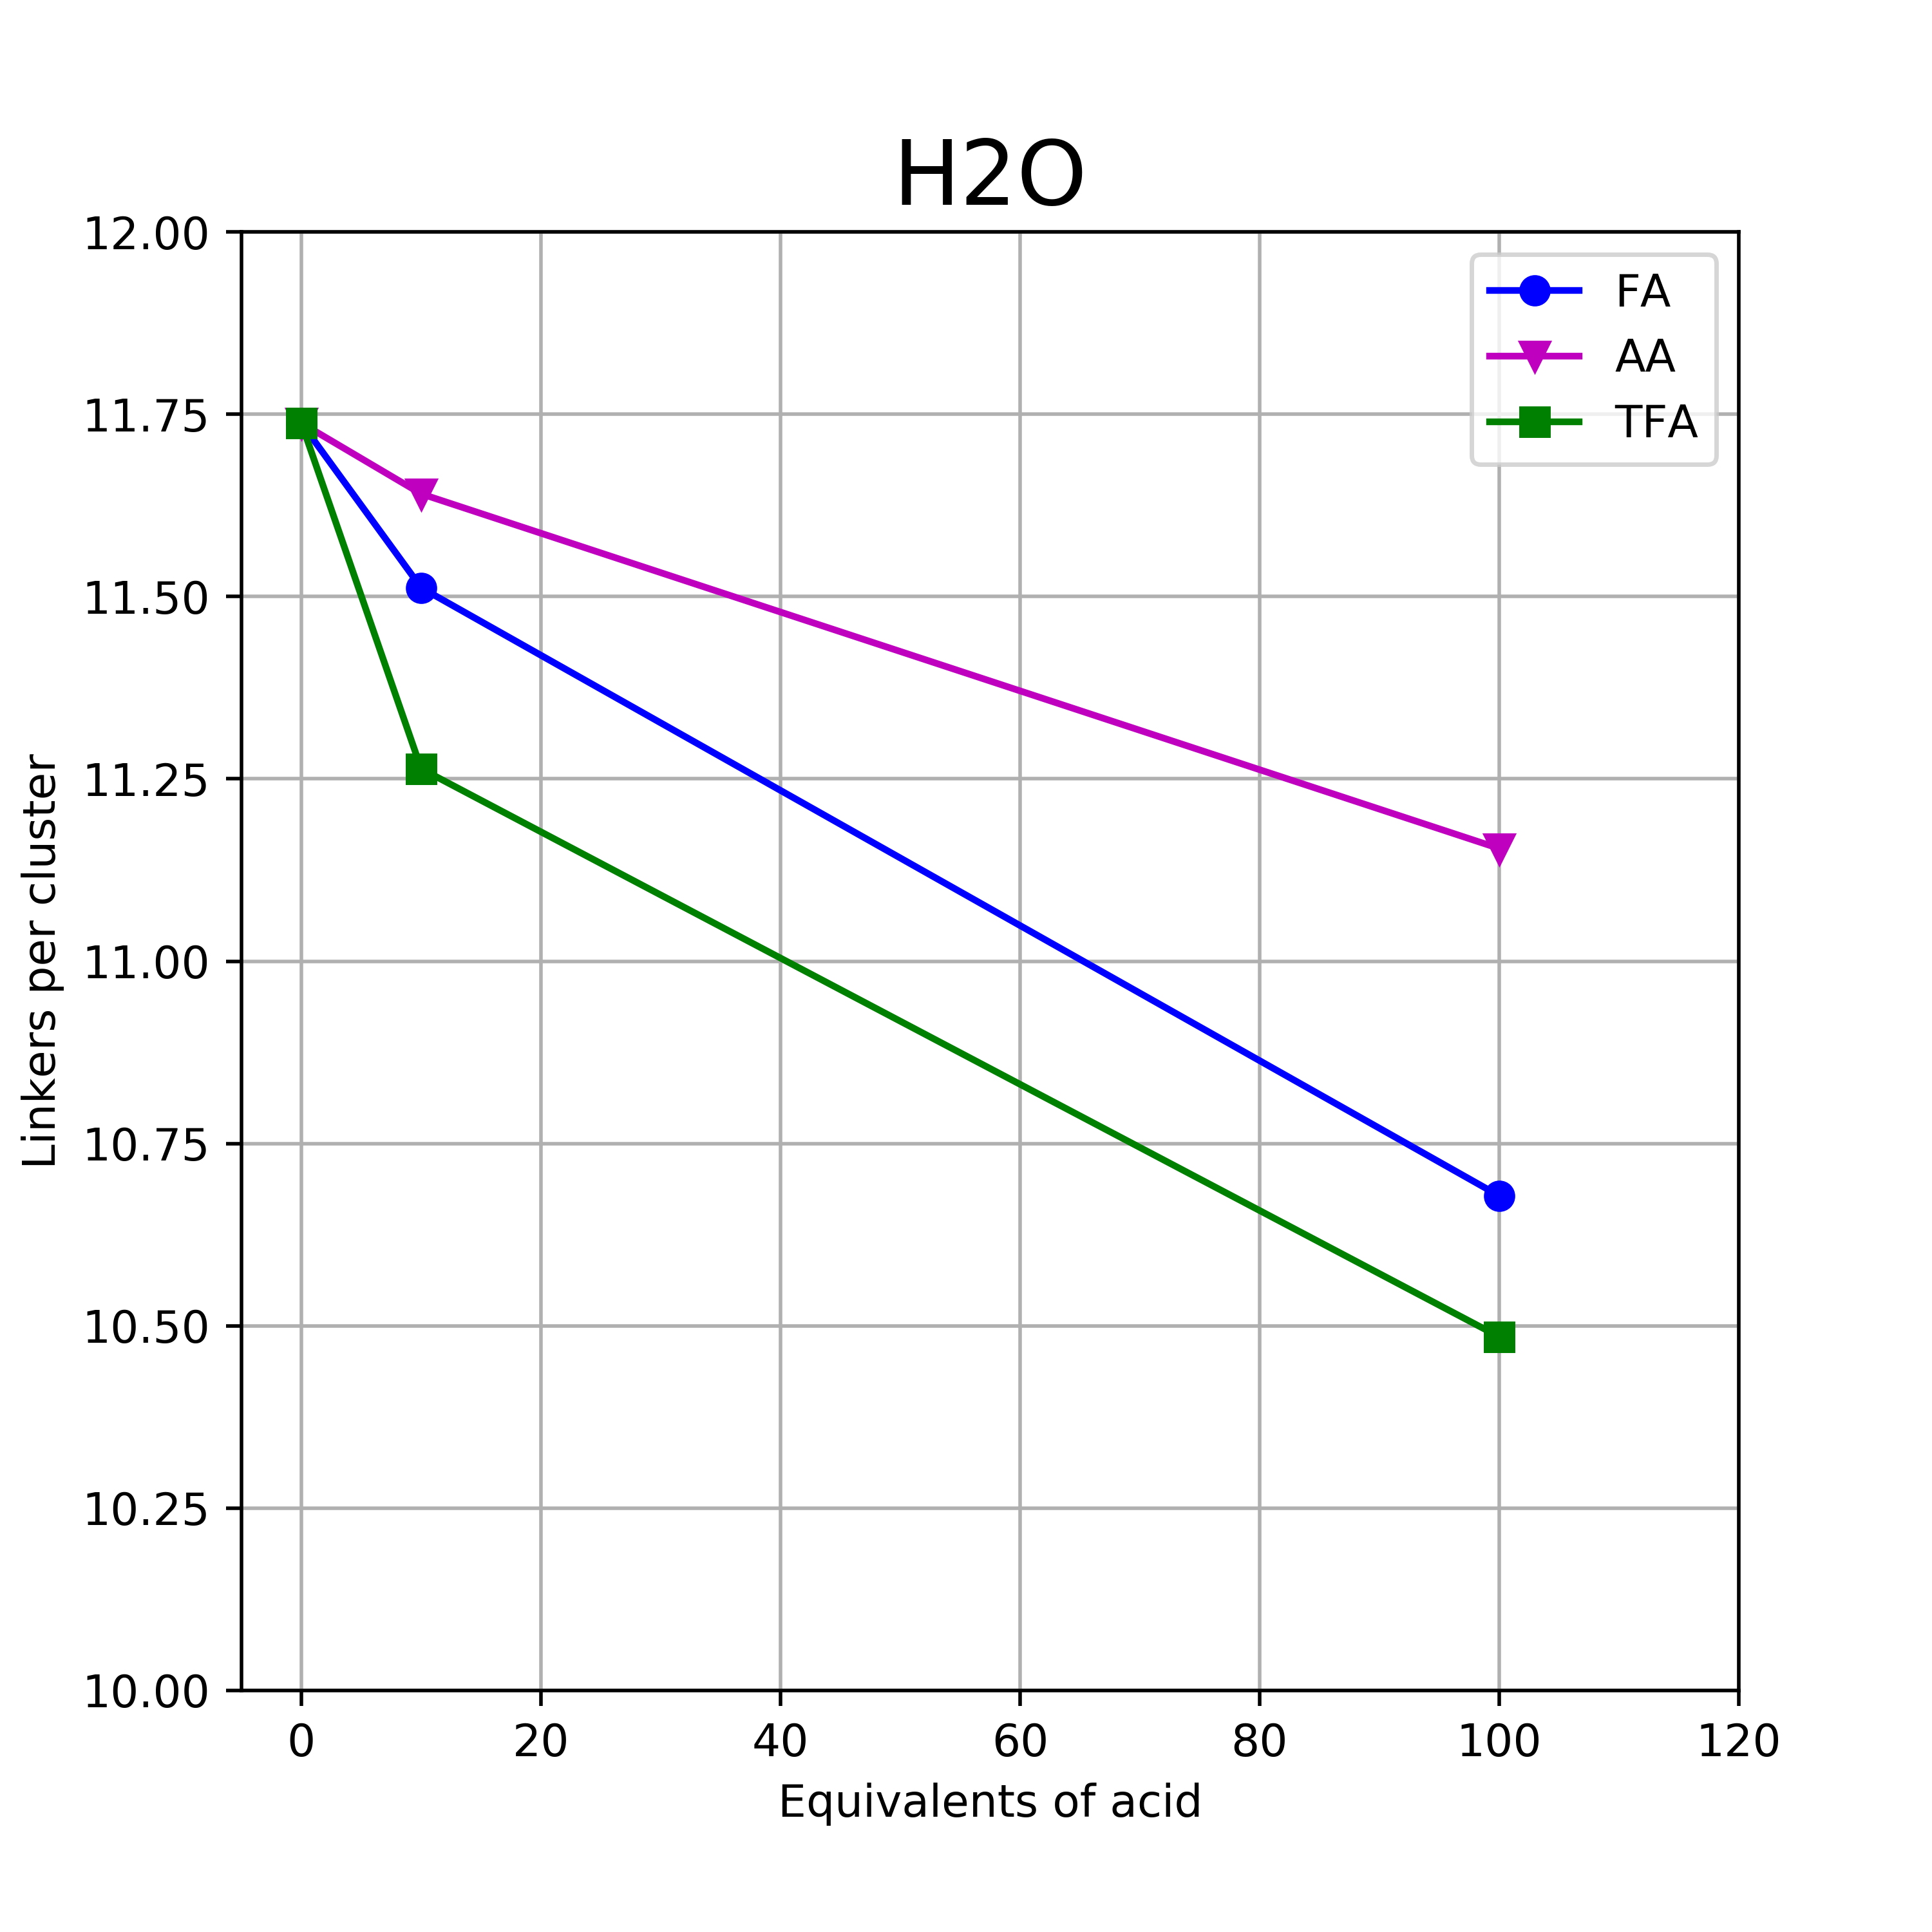
\includegraphics[width=\textwidth]{tga/H2O-def-overview}%
        \caption{}%
        \label{def:fgr:tga-h2o-linkers}
    \end{subfigure}%
    \begin{subfigure}{0.25\linewidth}
        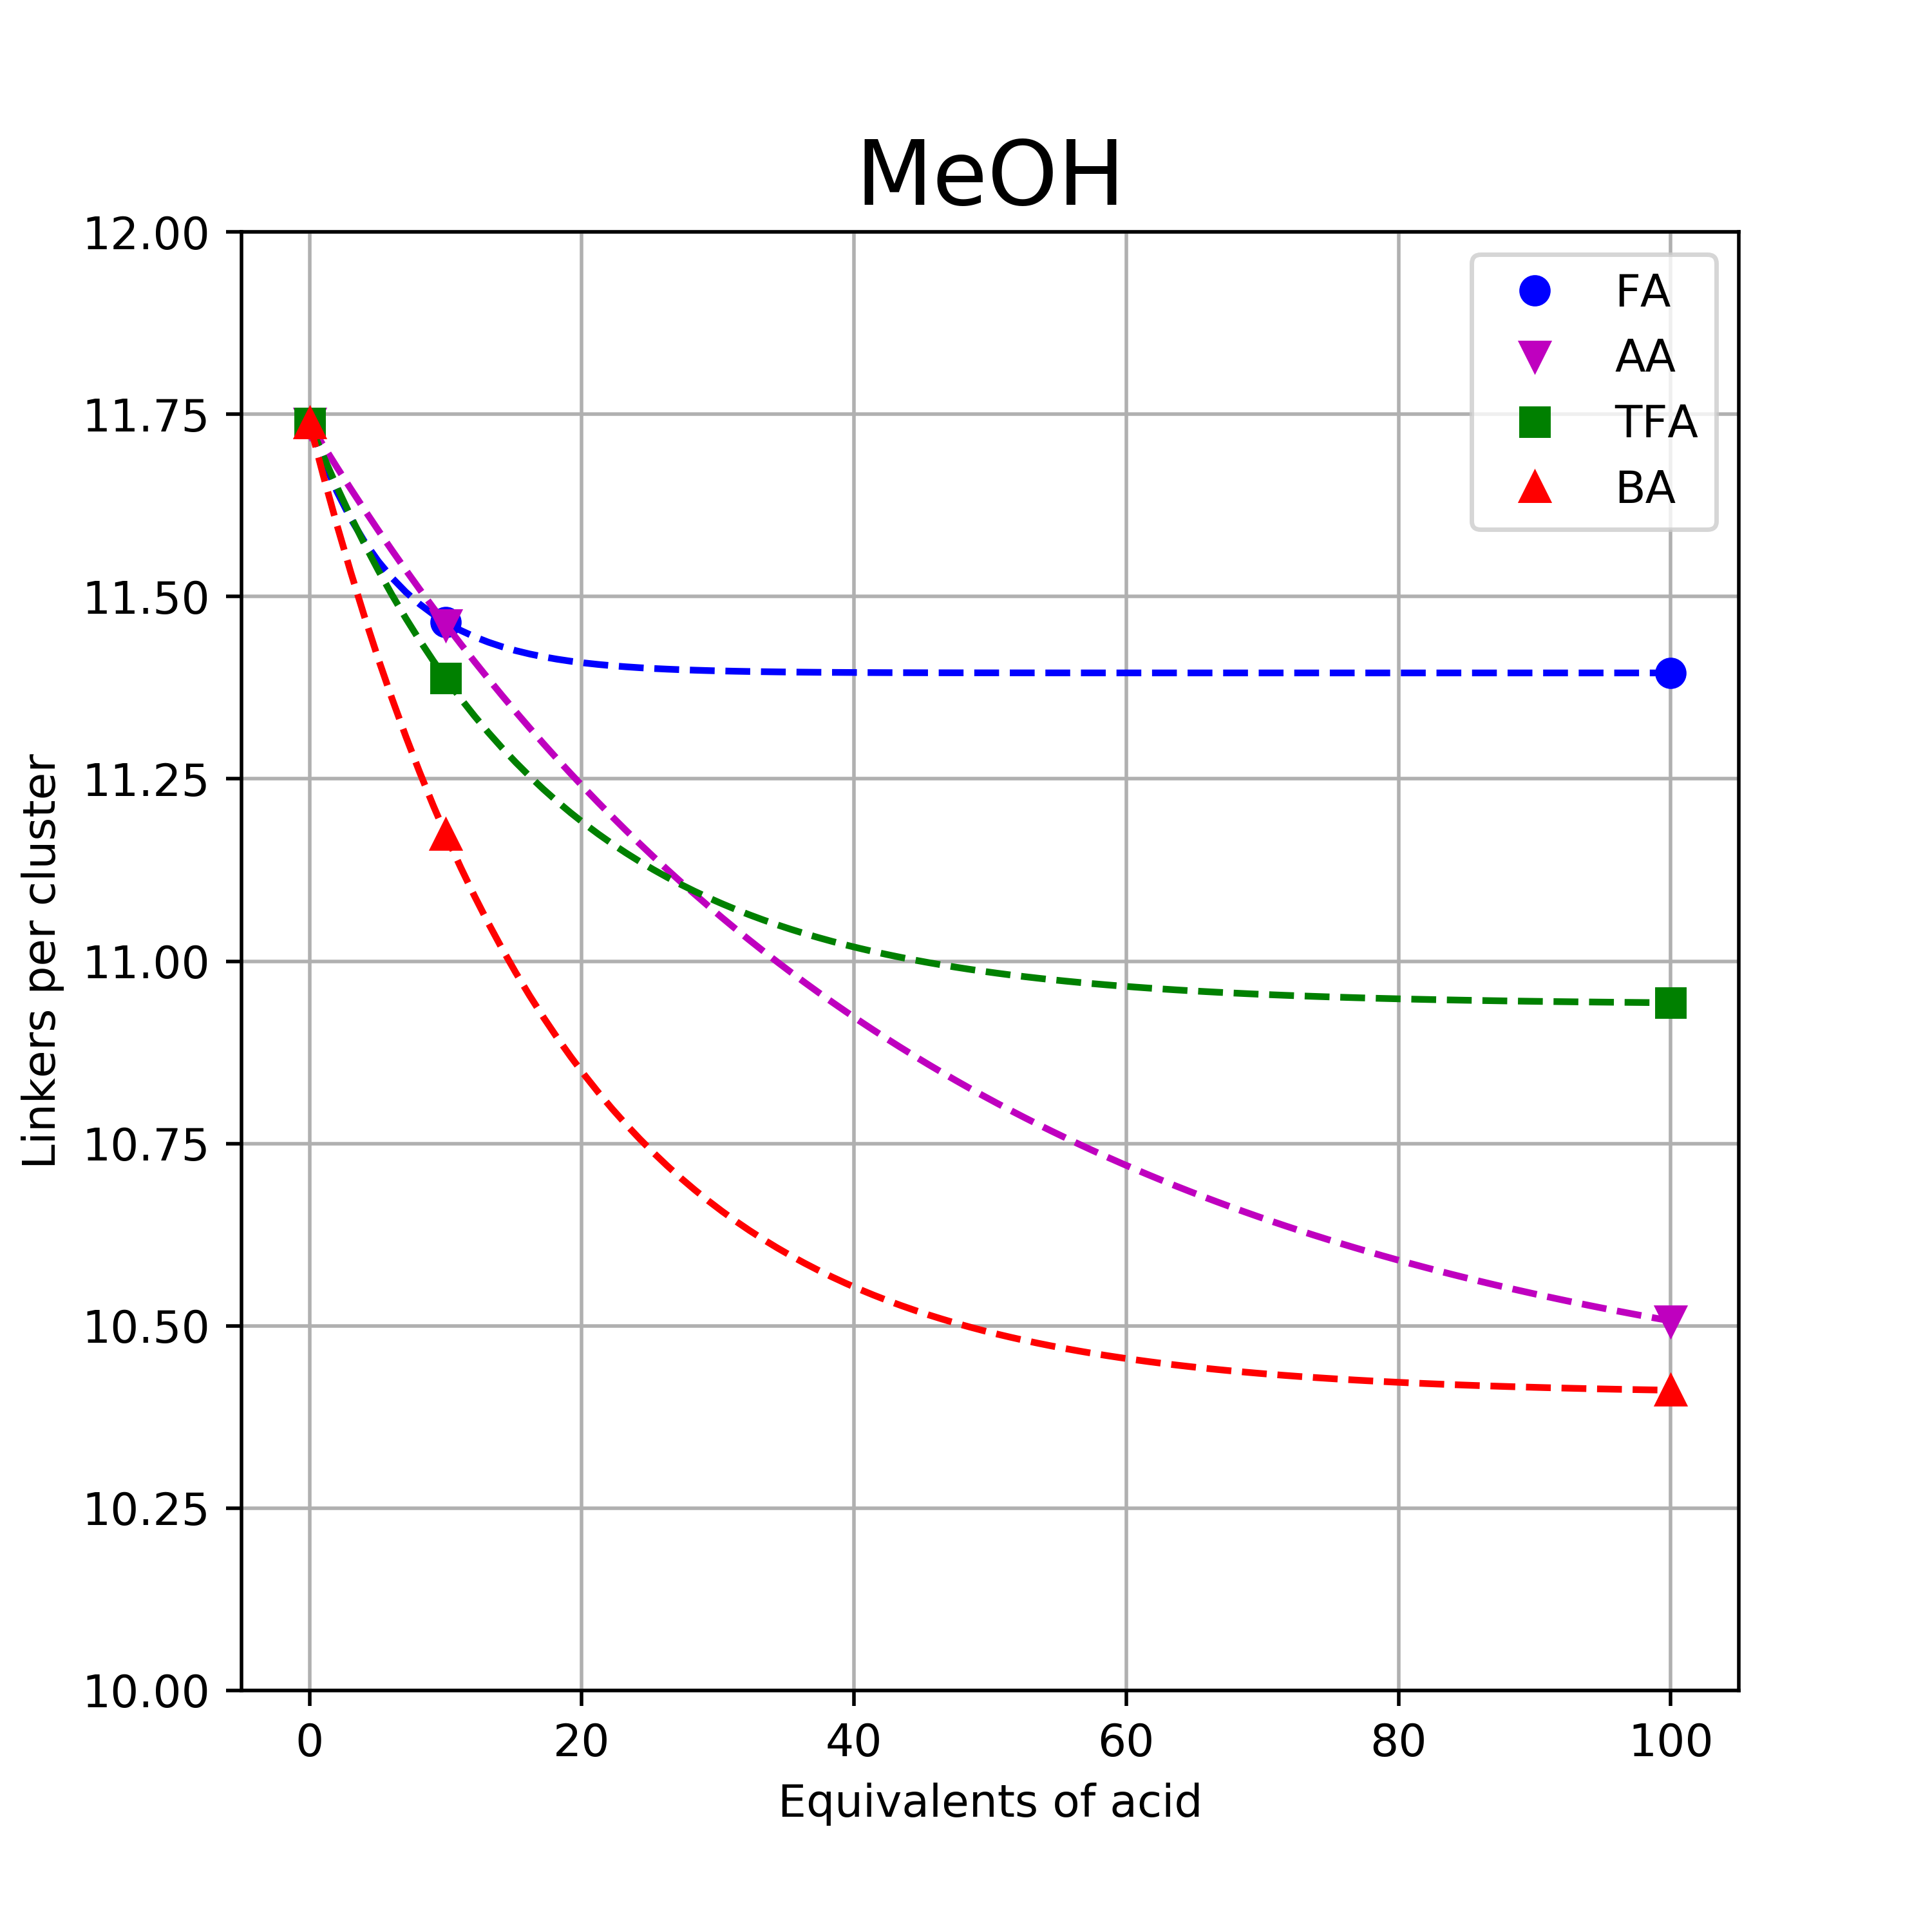
\includegraphics[width=\textwidth]{tga/MeOH-def-overview}%
        \caption{}%
        \label{def:fgr:tga-meoh-linkers}
    \end{subfigure}%
    \begin{subfigure}{0.25\linewidth}
        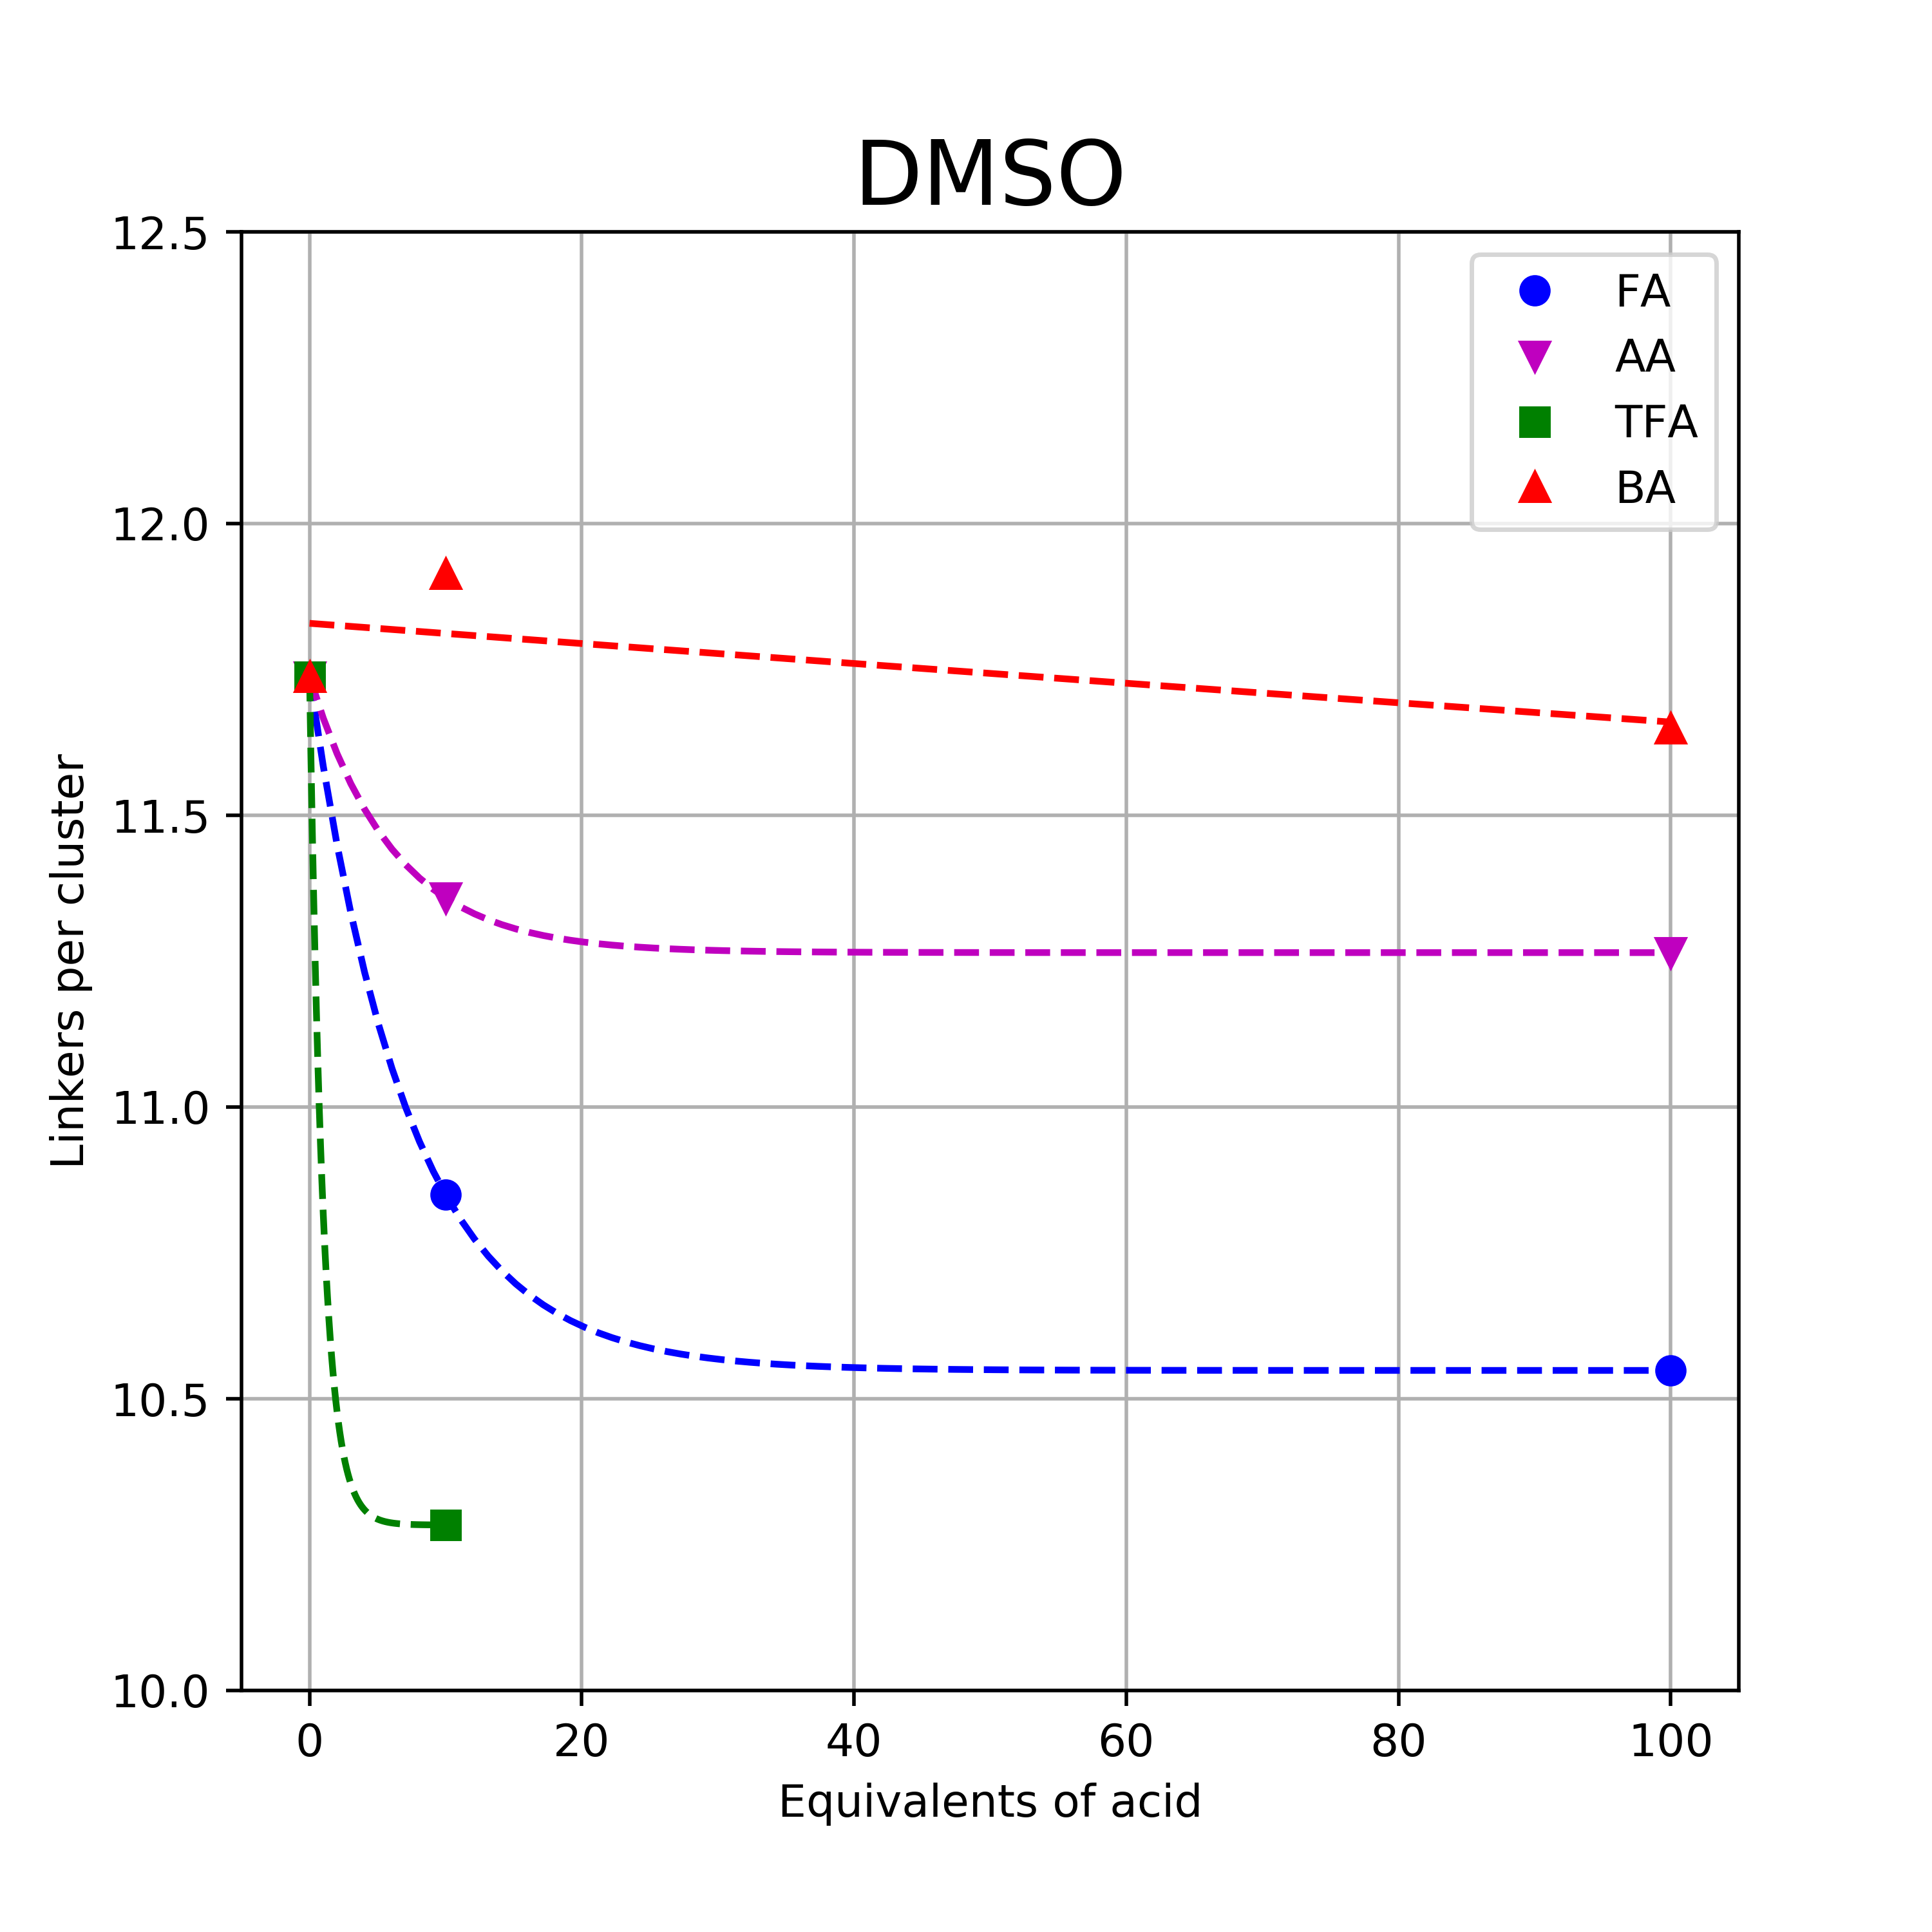
\includegraphics[width=\textwidth]{tga/DMSO-def-overview}%
        \caption{}%
        \label{def:fgr:tga-dmso-linkers}
    \end{subfigure}%

    \caption{Calculated linker-to-node ratio from the TGA curve 
    normalized mass at \SI{420}{\degreeCelsius} for (a) DMF 
    (b) \ce{H2O}, (c) \ce{MeOH} and (d) DMSO leached samples.
    A ratio of 12 to 1 corresponds to a completely defect-free
    structure. An exponential decay trendline is fitted to 
    each set of points.}%
    \label{def:fgr:tga-defects}
    
\end{figure}

For the nitrogen adsorption dataset, the predictors described in the 
previous section have been calculated using the pyGAPS framework
(\autoref{pyg}). The Henry constant is determined through the 
initial slope method, with a linear section found below 
\(10^{-4}~p/p_0\). Pore volume is taken as the liquid density
of the amount adsorbed at \(0.8~p/p_0\), assuming that the 
nitrogen is in a liquid-like state in the MOF pores. The pore
size distribution was calculated through the Horvatz-Kawazoe
method for micropores, the Dollimore-Heal method for mesopores
and DFT kernel fitting for a multiscale distribution. While 
the applicability of these methods for determination of absolute
pore size is doubtful, they can provide comparisons between 
different samples of the same material.

\begin{figure}[htb]
    \centering

    \begin{subfigure}{0.25\linewidth}
        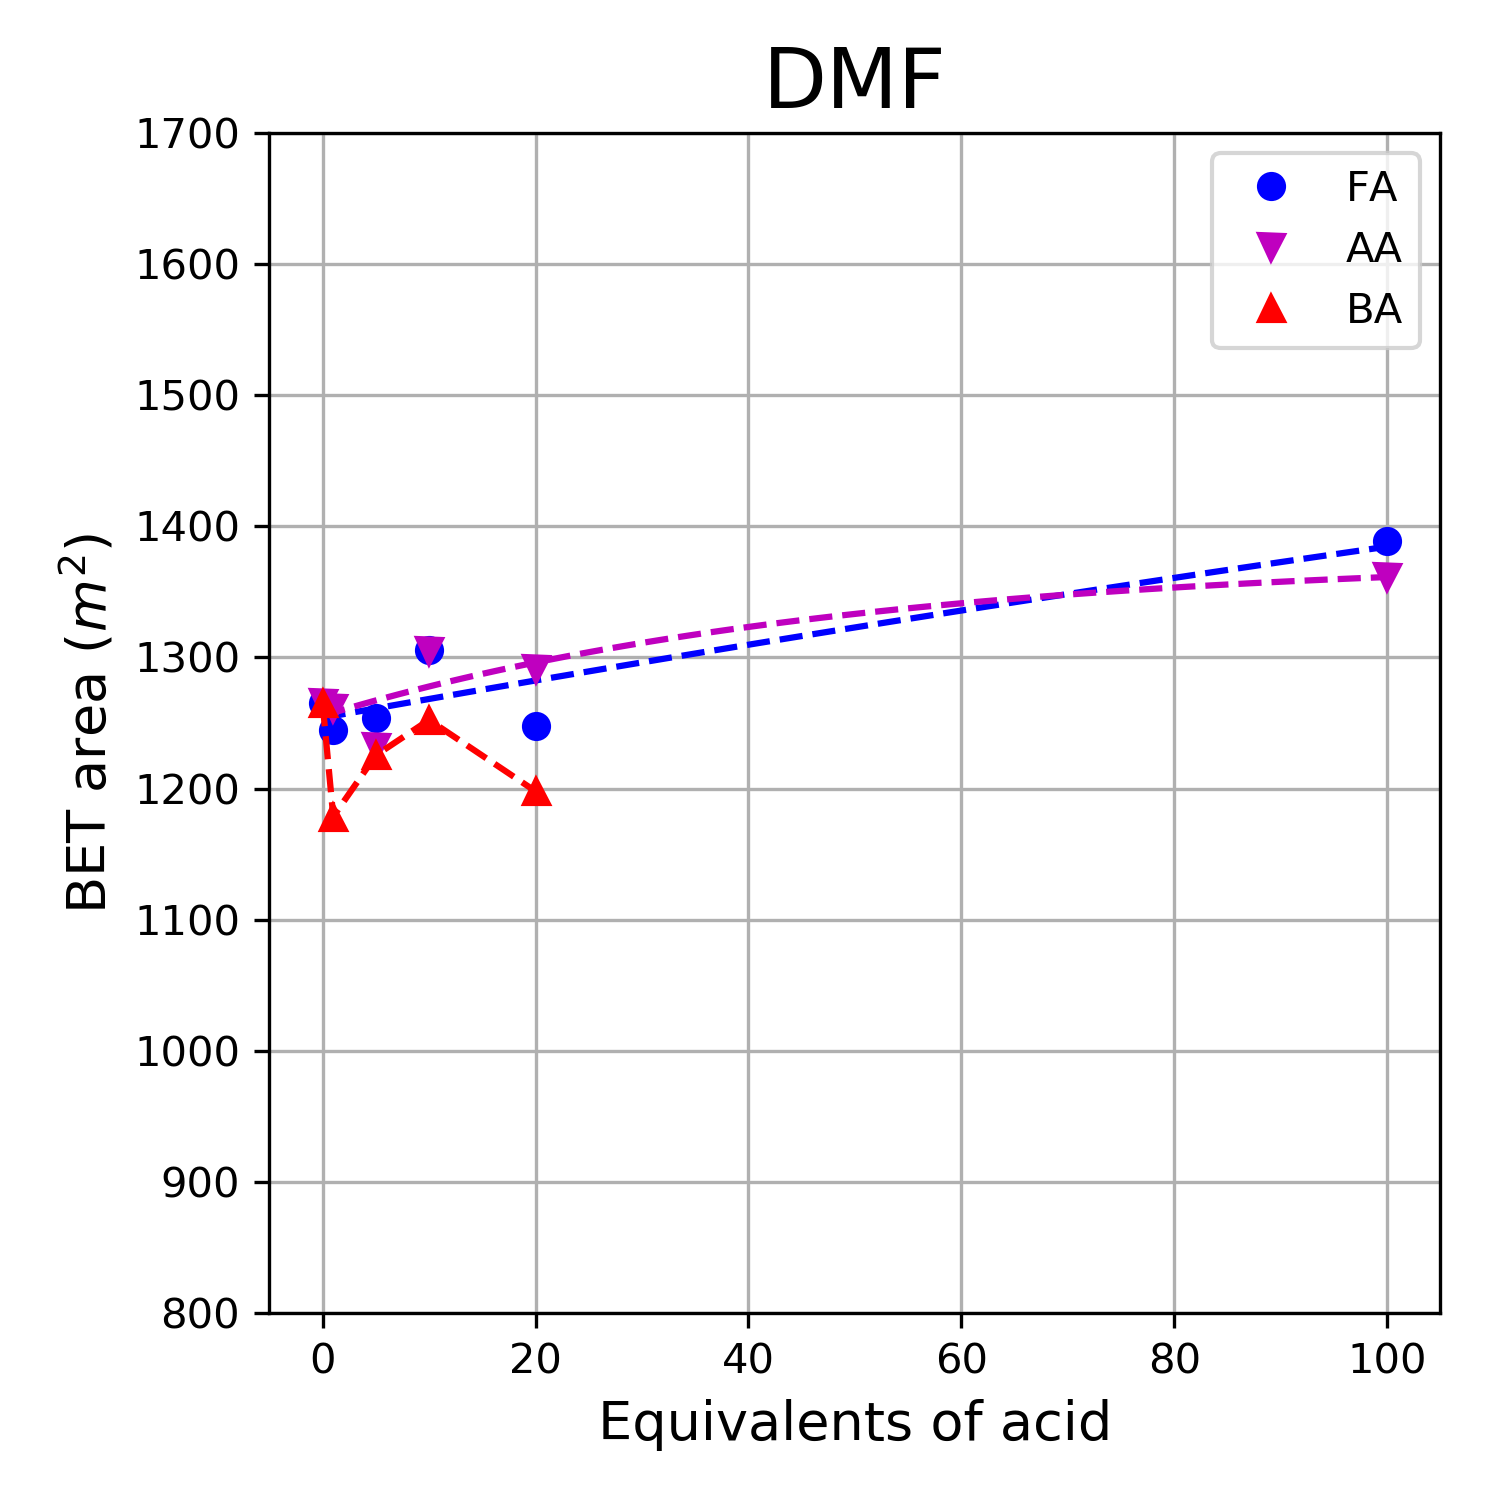
\includegraphics[width=\textwidth]{n2phys/dmf-area}%
        \caption{}%
        \label{def:fgr:n2phys-dmf-area}
    \end{subfigure}%
    \begin{subfigure}{0.25\linewidth}
        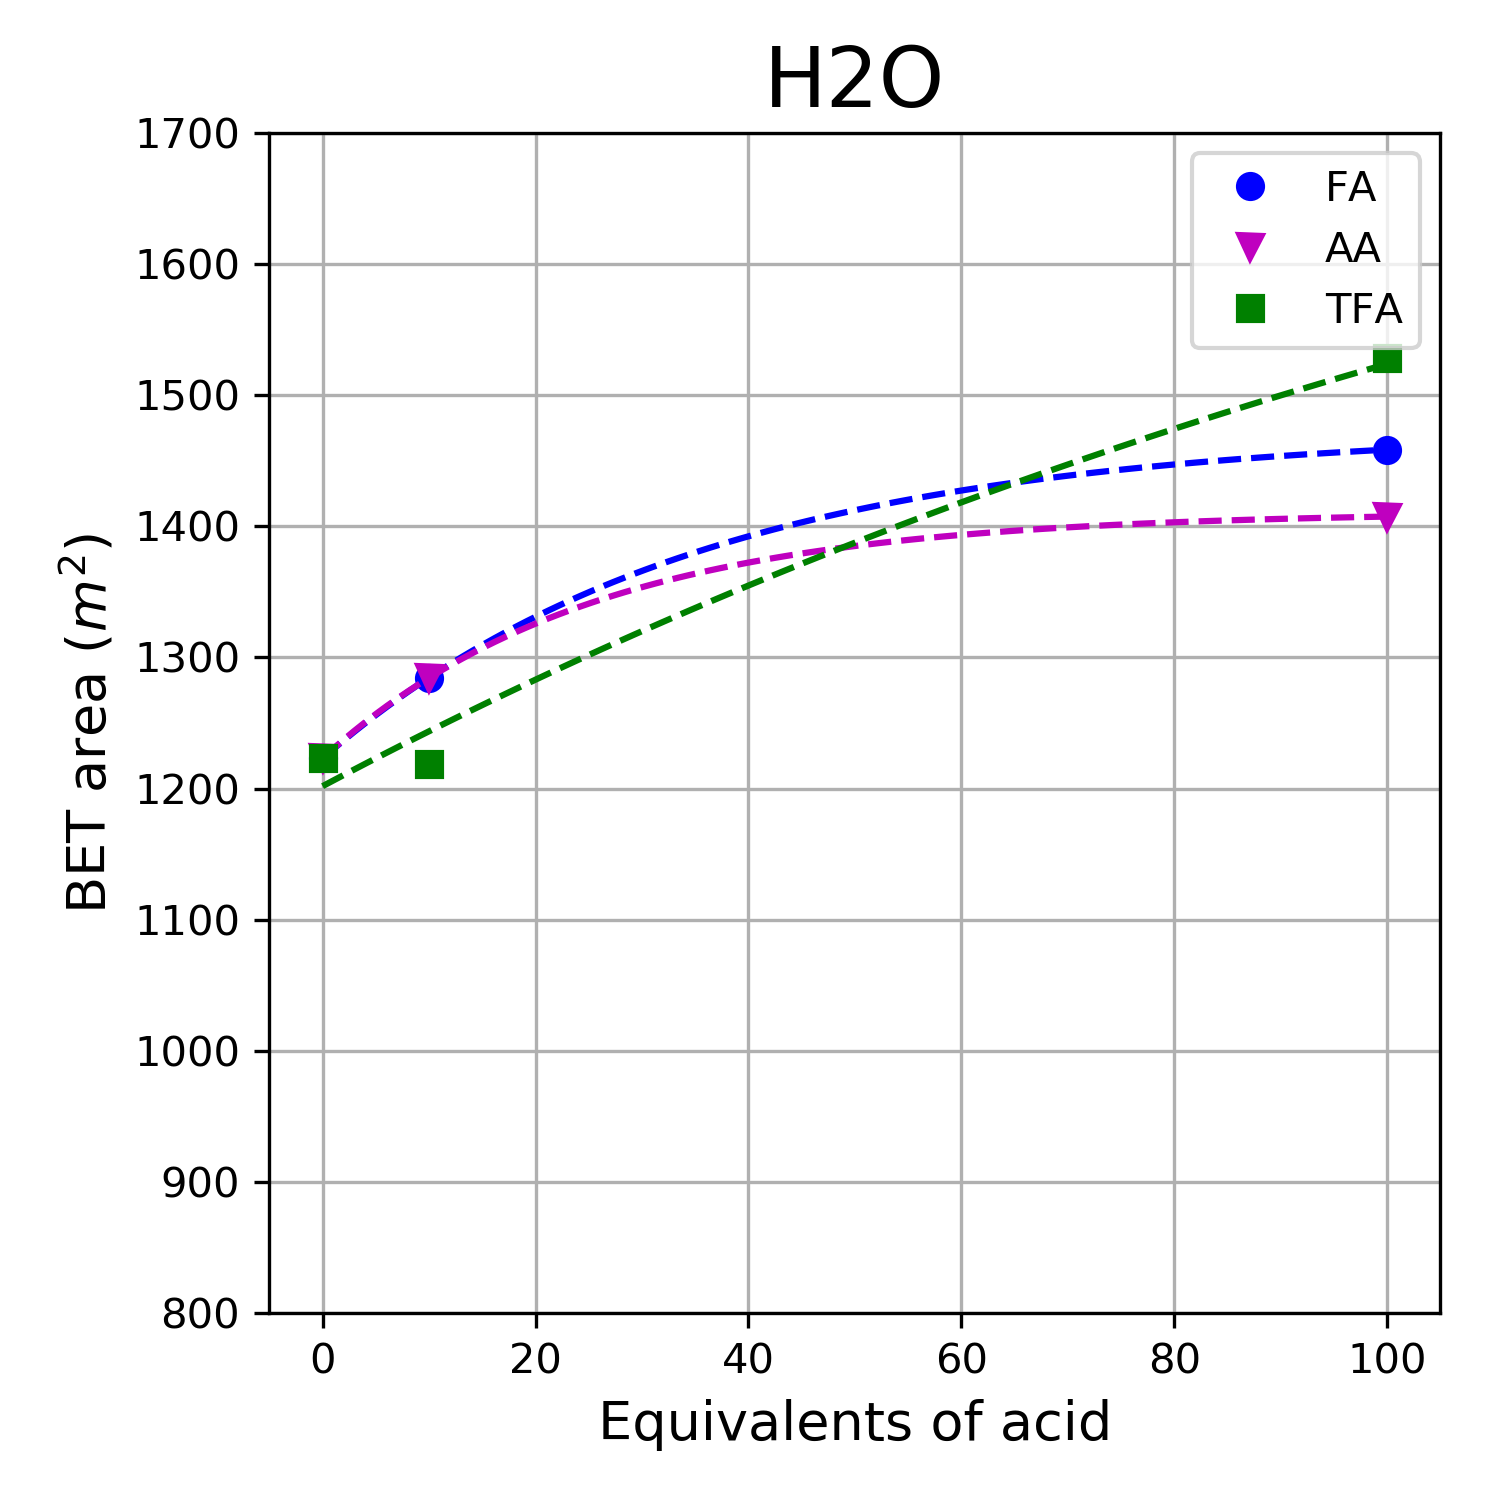
\includegraphics[width=\textwidth]{n2phys/h2o-area}%
        \caption{}%
        \label{def:fgr:n2phys-h2o-area}
    \end{subfigure}%
    \begin{subfigure}{0.25\linewidth}
        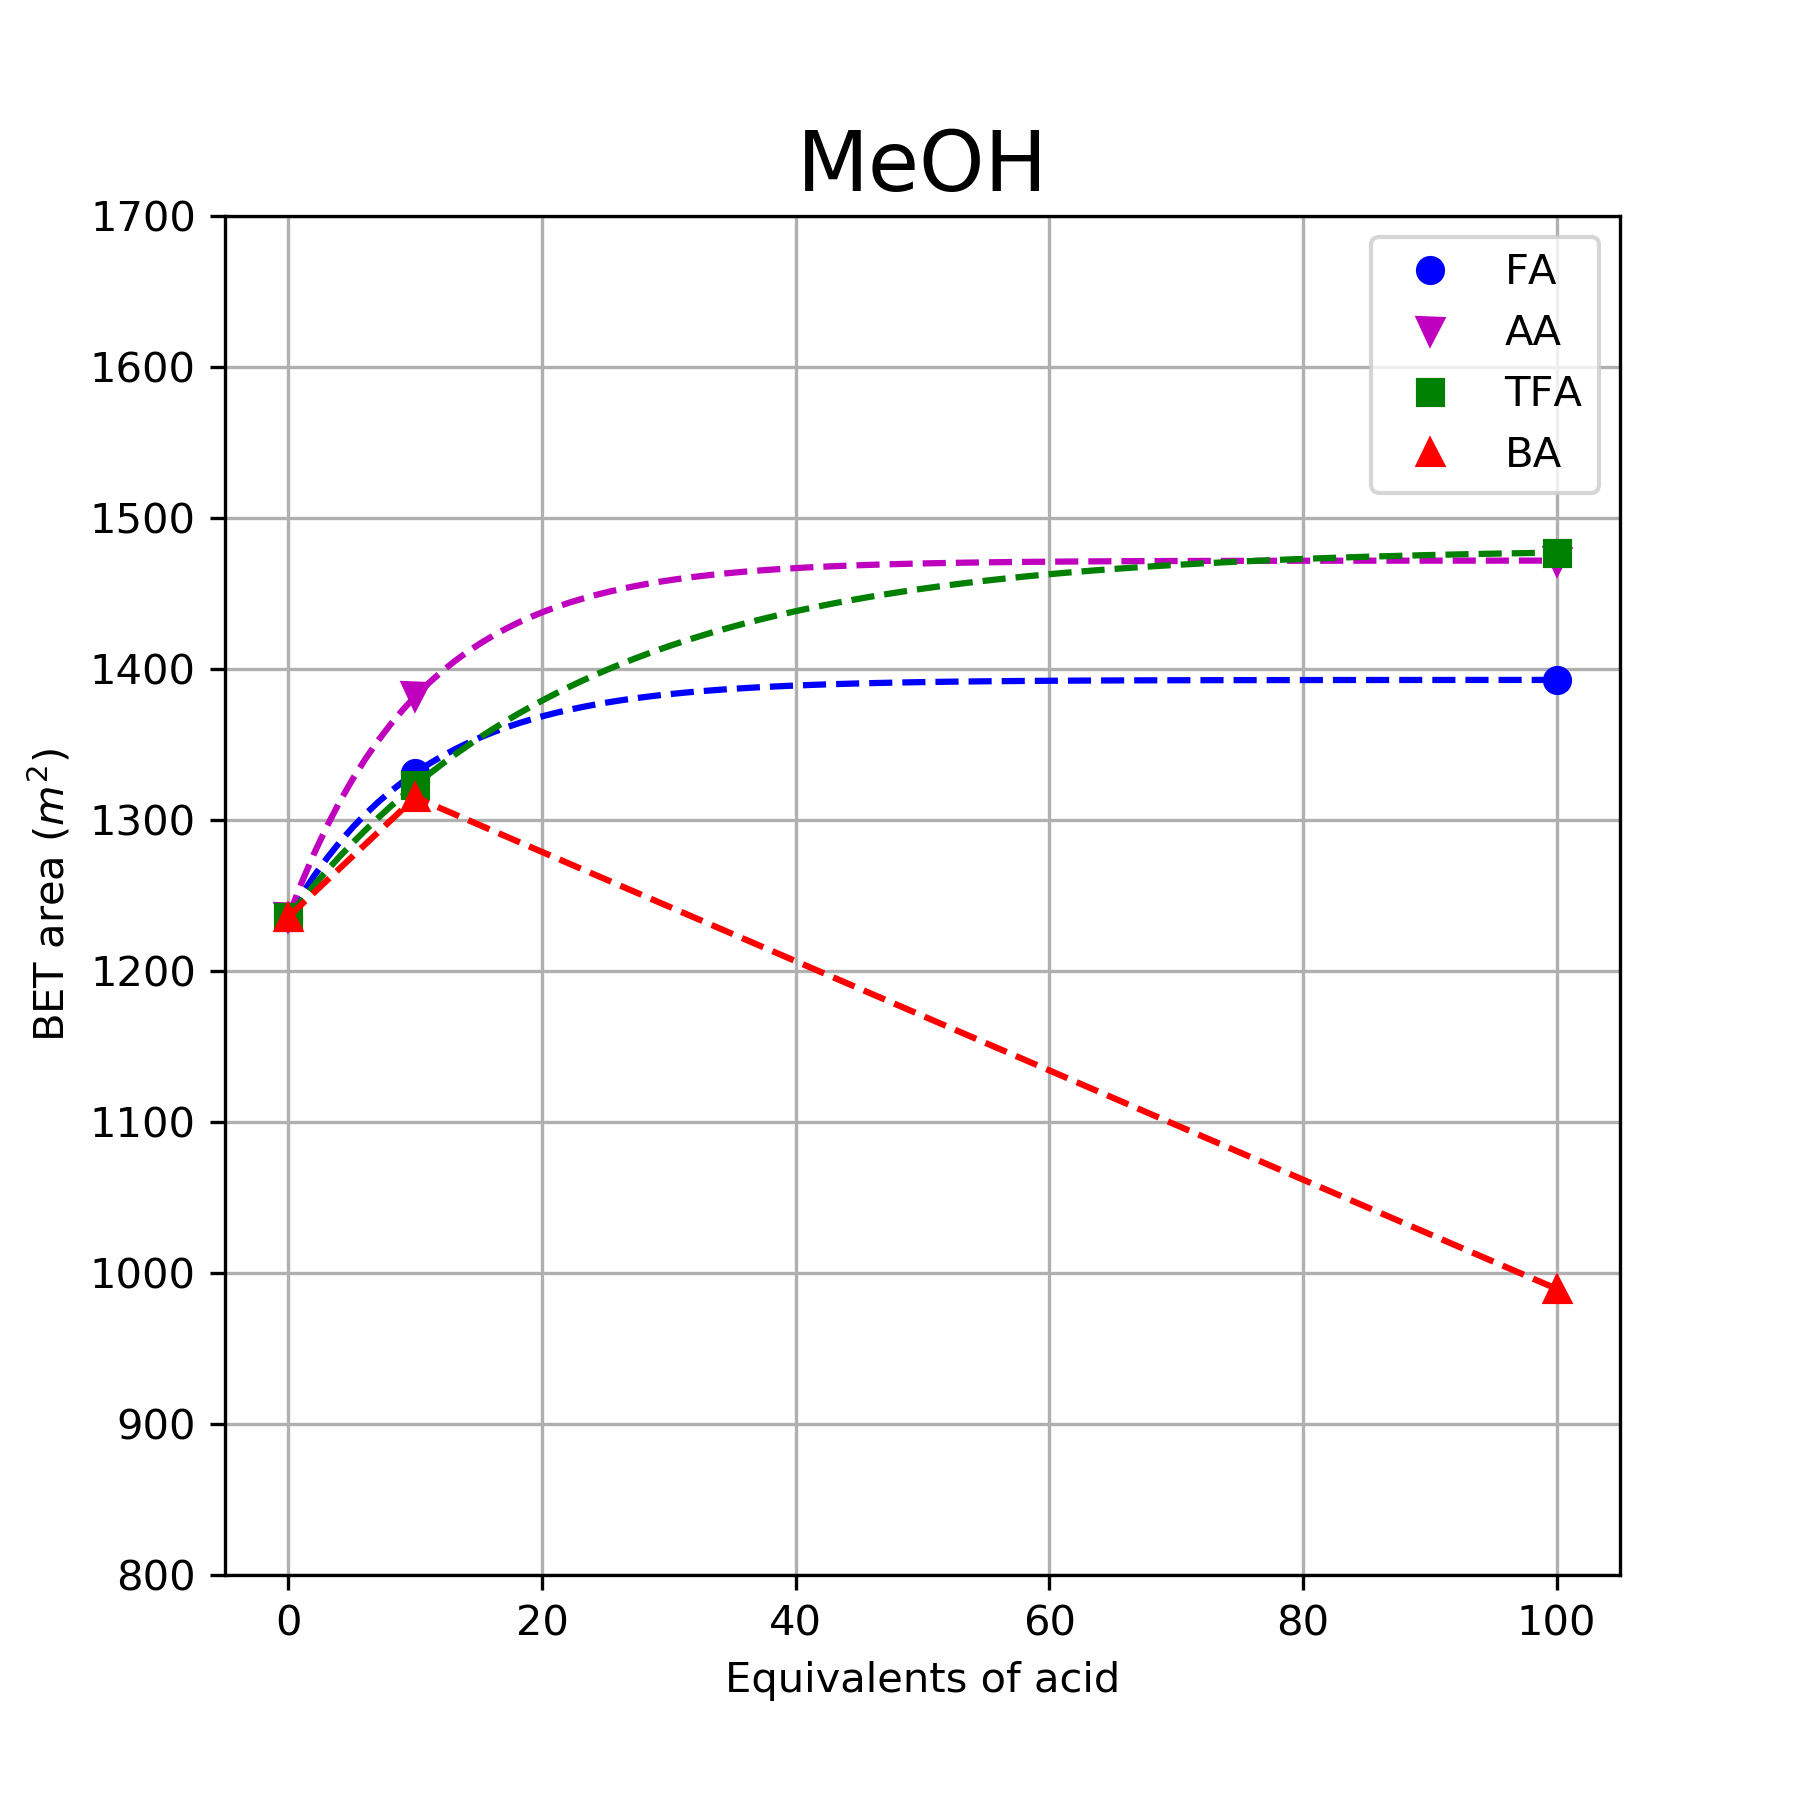
\includegraphics[width=\textwidth]{n2phys/meoh-area}%
        \caption{}%
        \label{def:fgr:n2phys-meoh-area}
    \end{subfigure}%
    \begin{subfigure}{0.25\linewidth}
        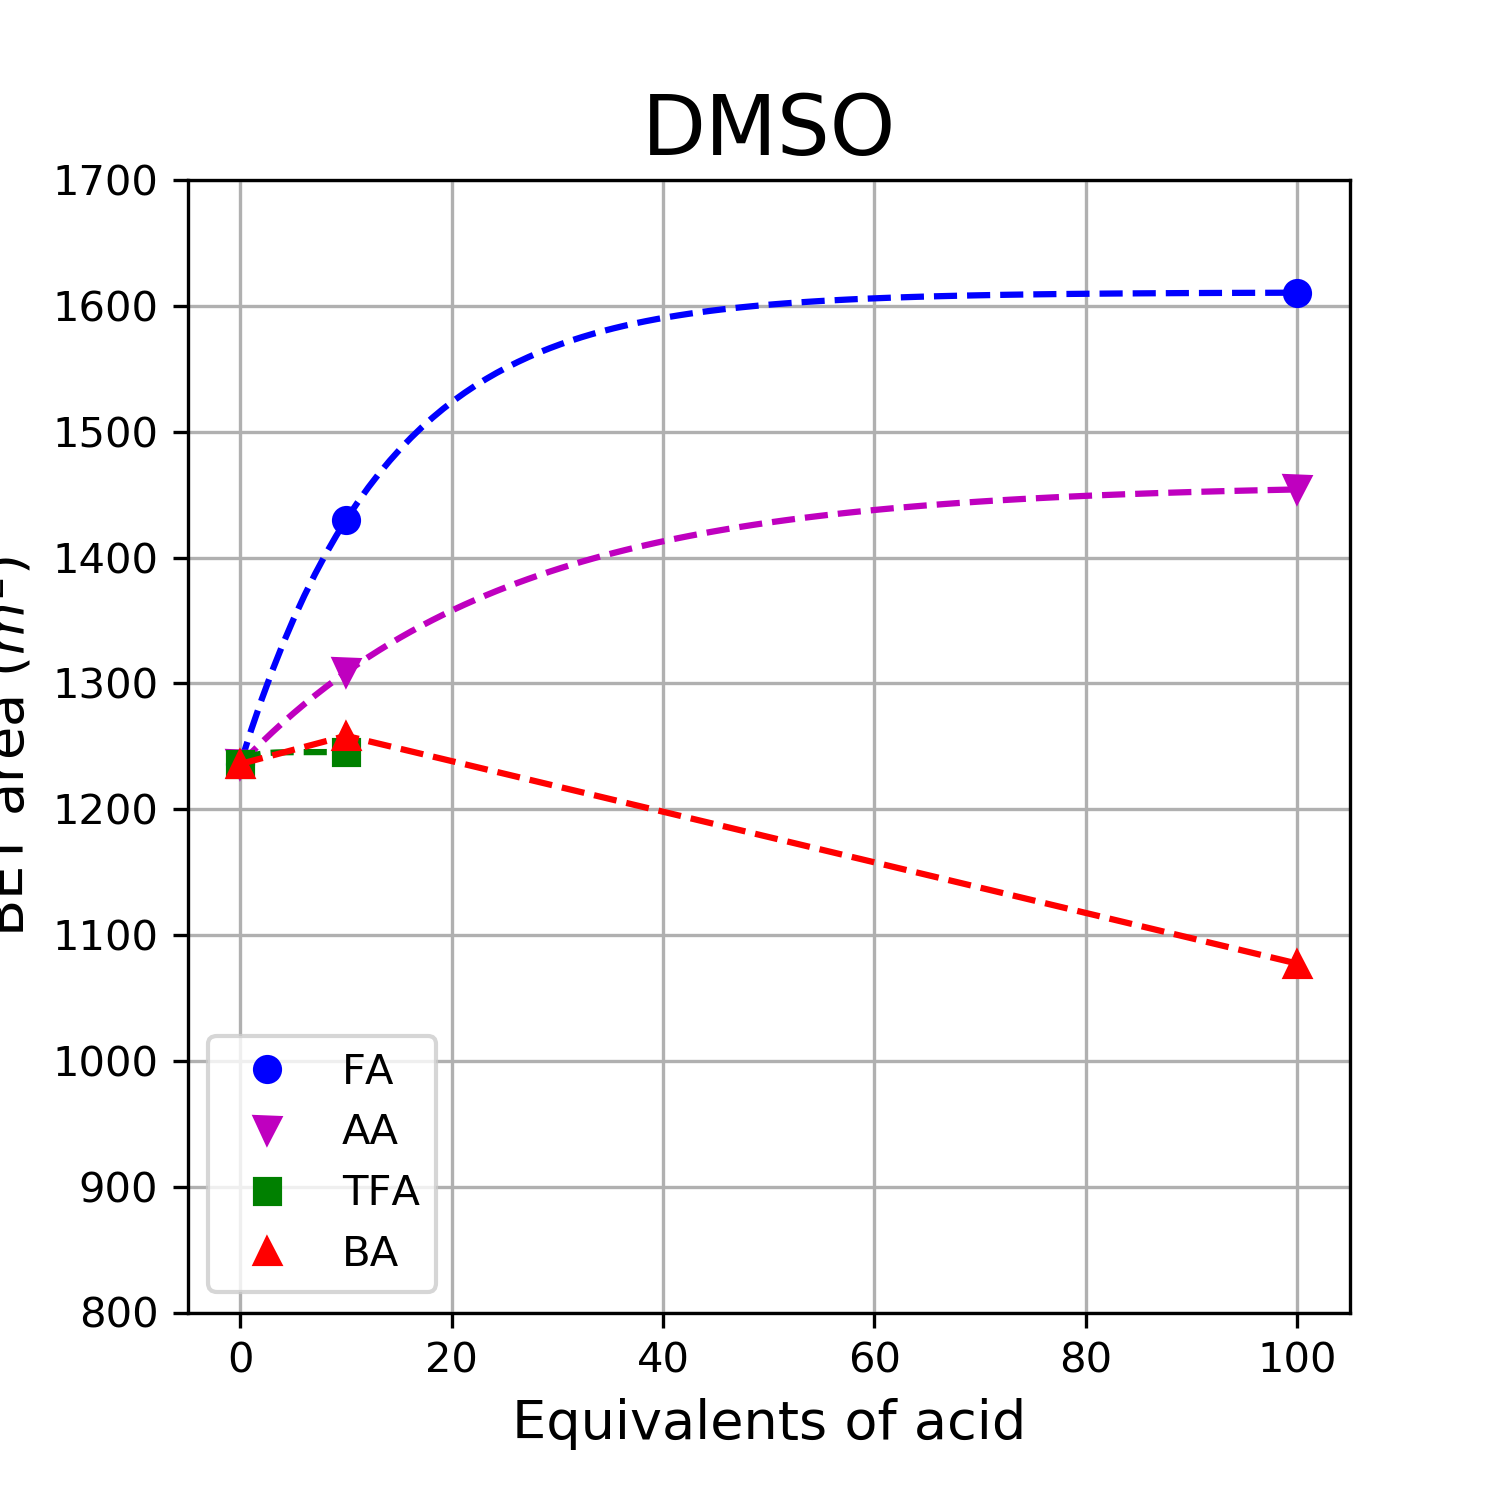
\includegraphics[width=\textwidth]{n2phys/dmso-area}%
        \caption{}%
        \label{def:fgr:n2phys-dmso-area}
    \end{subfigure}%

    \begin{subfigure}{0.25\linewidth}
        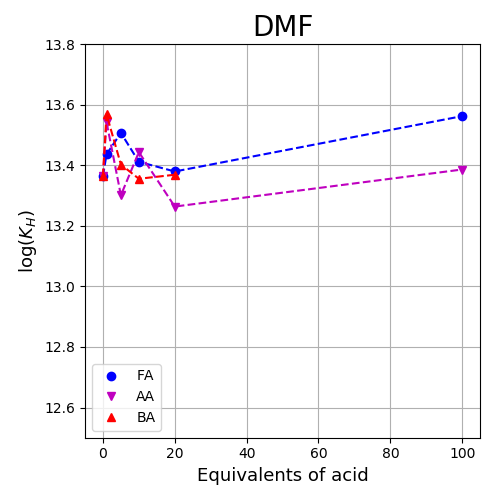
\includegraphics[width=\textwidth]{n2phys/dmf-henry}%
        \caption{}%
        \label{def:fgr:n2phys-dmf-henry}
    \end{subfigure}%
    \begin{subfigure}{0.25\linewidth}
        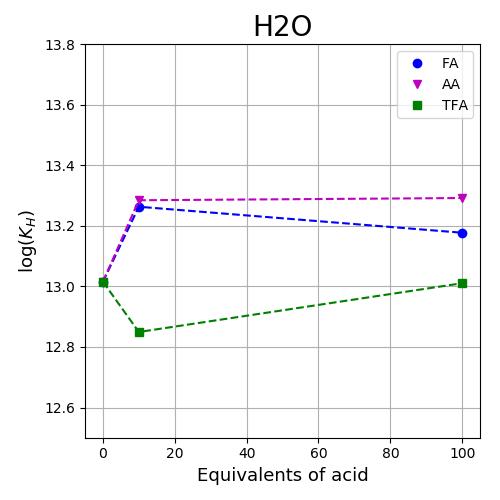
\includegraphics[width=\textwidth]{n2phys/h2o-henry}%
        \caption{}%
        \label{def:fgr:n2phys-h2o-henry}
    \end{subfigure}%
    \begin{subfigure}{0.25\linewidth}
        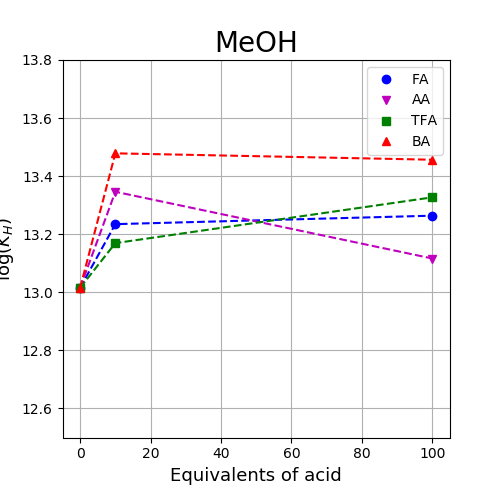
\includegraphics[width=\textwidth]{n2phys/meoh-henry}%
        \caption{}%
        \label{def:fgr:n2phys-meoh-henry}
    \end{subfigure}%
    \begin{subfigure}{0.25\linewidth}
        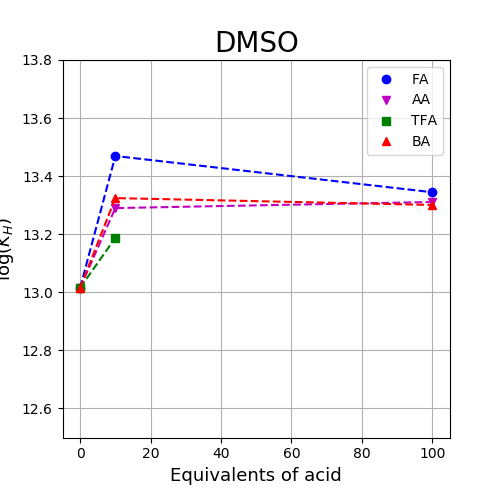
\includegraphics[width=\textwidth]{n2phys/dmso-henry}%
        \caption{}%
        \label{def:fgr:n2phys-dmso-henry}
    \end{subfigure}%

    \begin{subfigure}{0.25\linewidth}
        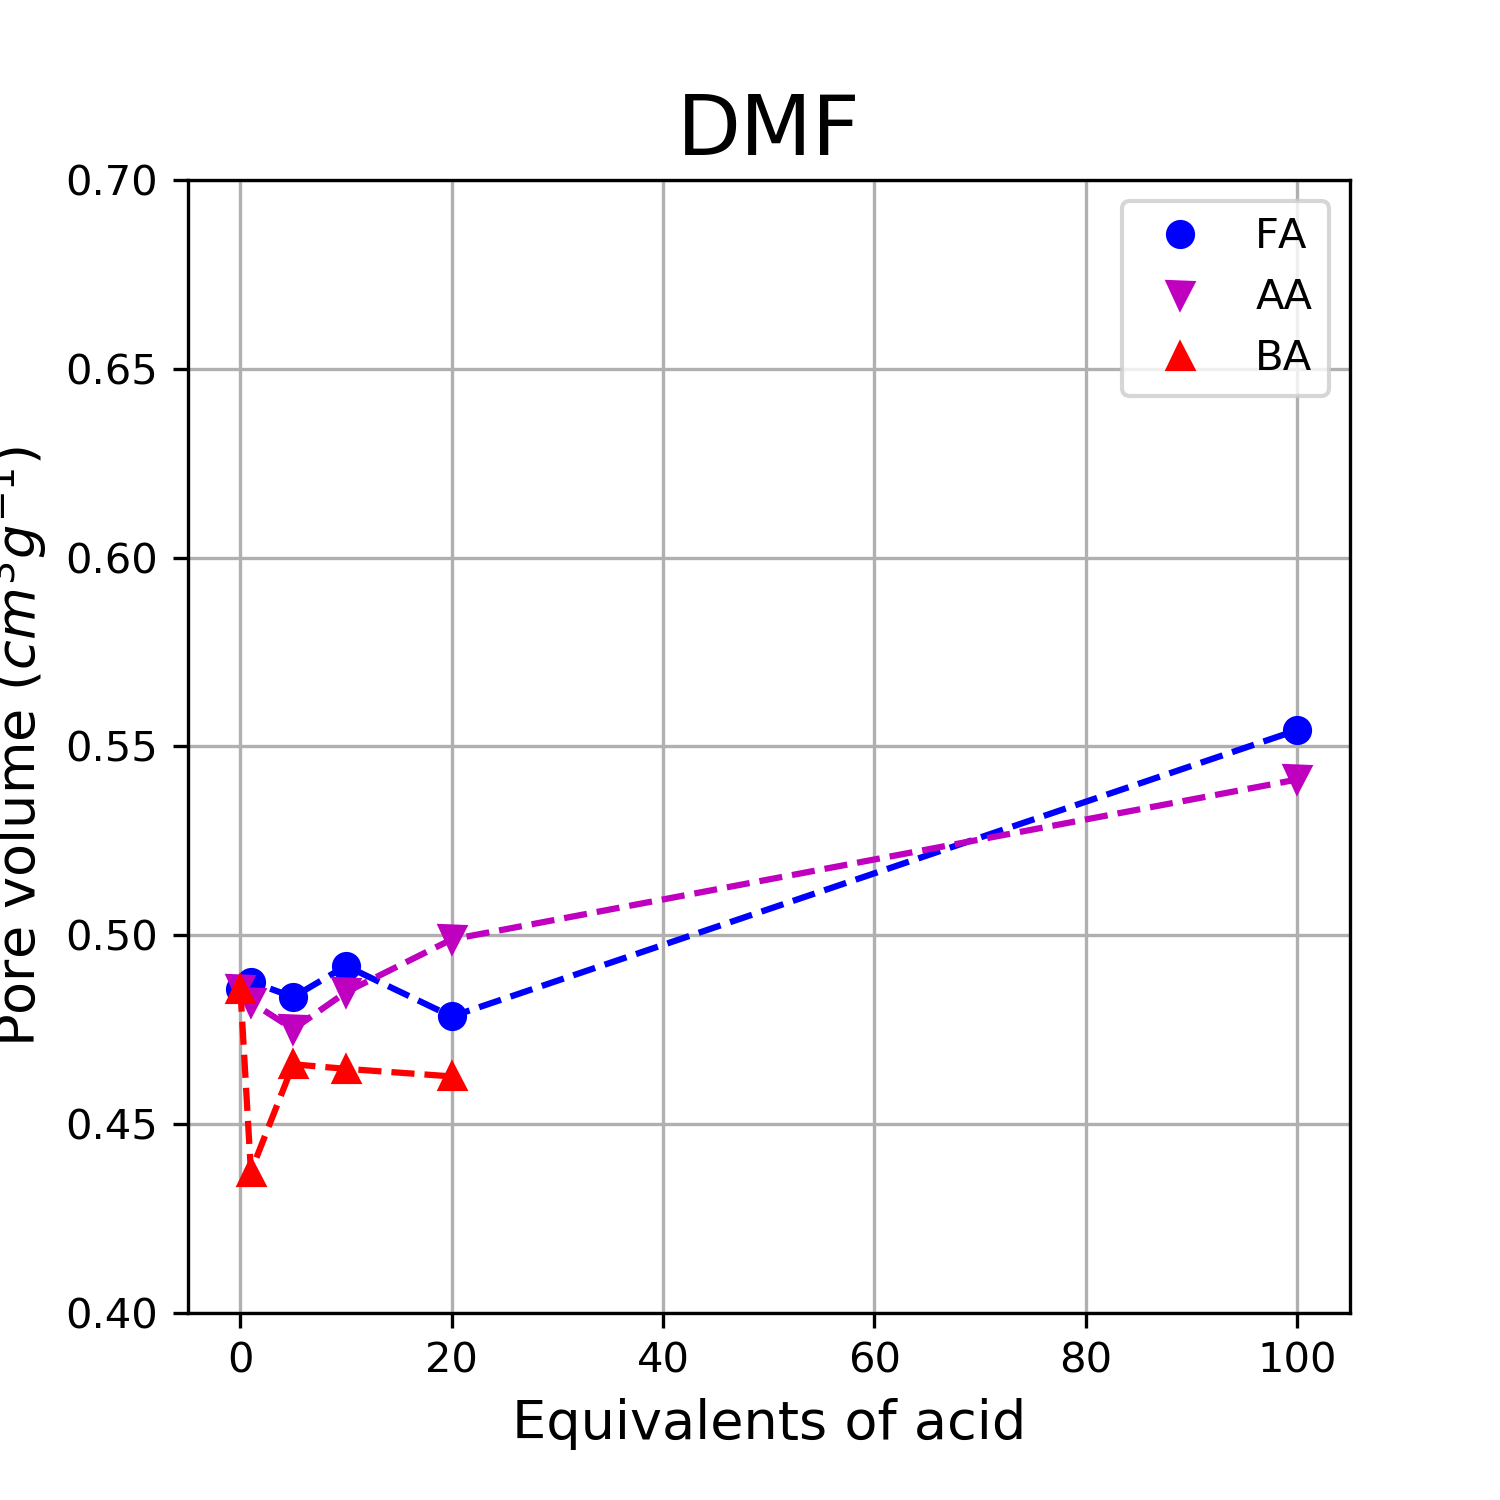
\includegraphics[width=\textwidth]{n2phys/dmf-porevol}%
        \caption{}%
        \label{def:fgr:n2phys-dmf-porevol}
    \end{subfigure}%
    \begin{subfigure}{0.25\linewidth}
        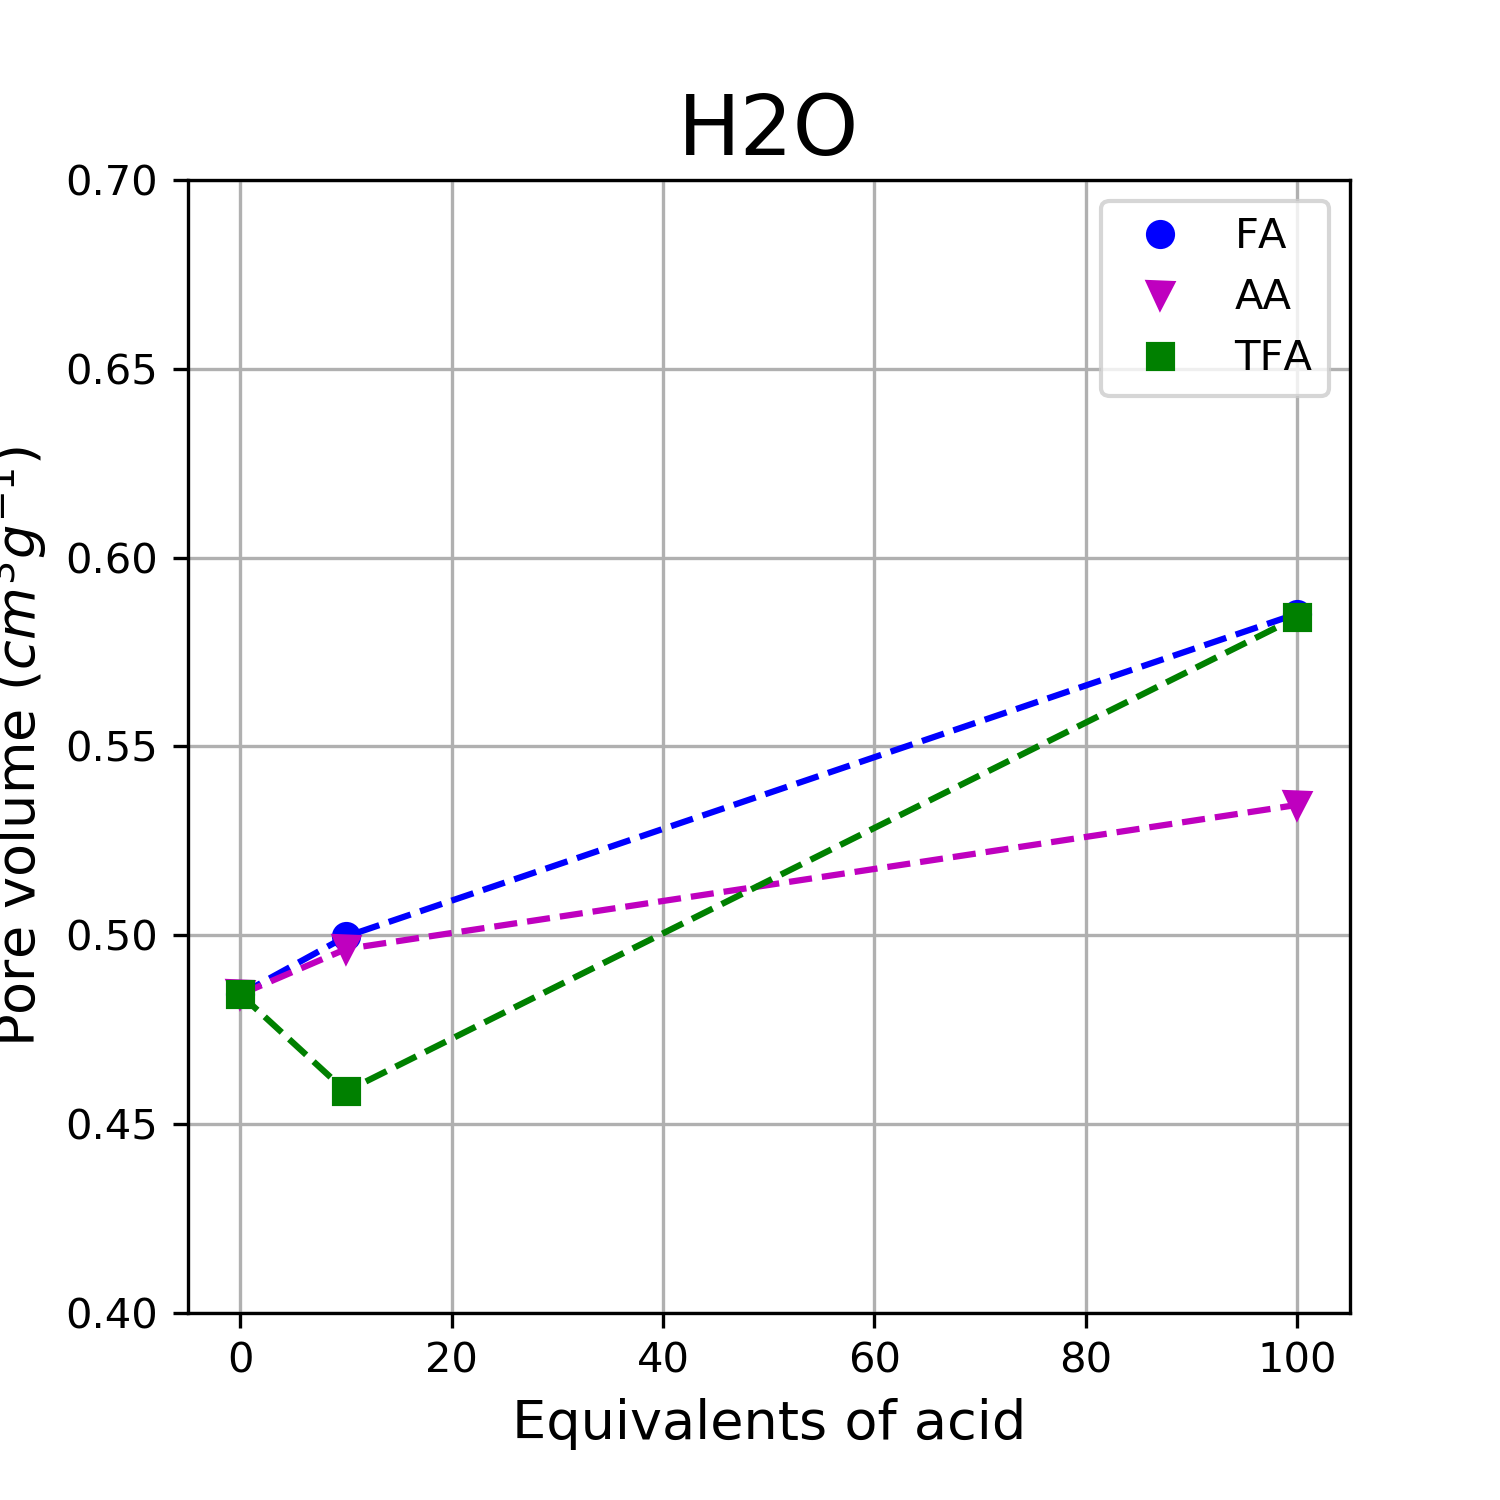
\includegraphics[width=\textwidth]{n2phys/h2o-porevol}%
        \caption{}%
        \label{def:fgr:n2phys-h2o-porevol}
    \end{subfigure}%
    \begin{subfigure}{0.25\linewidth}
        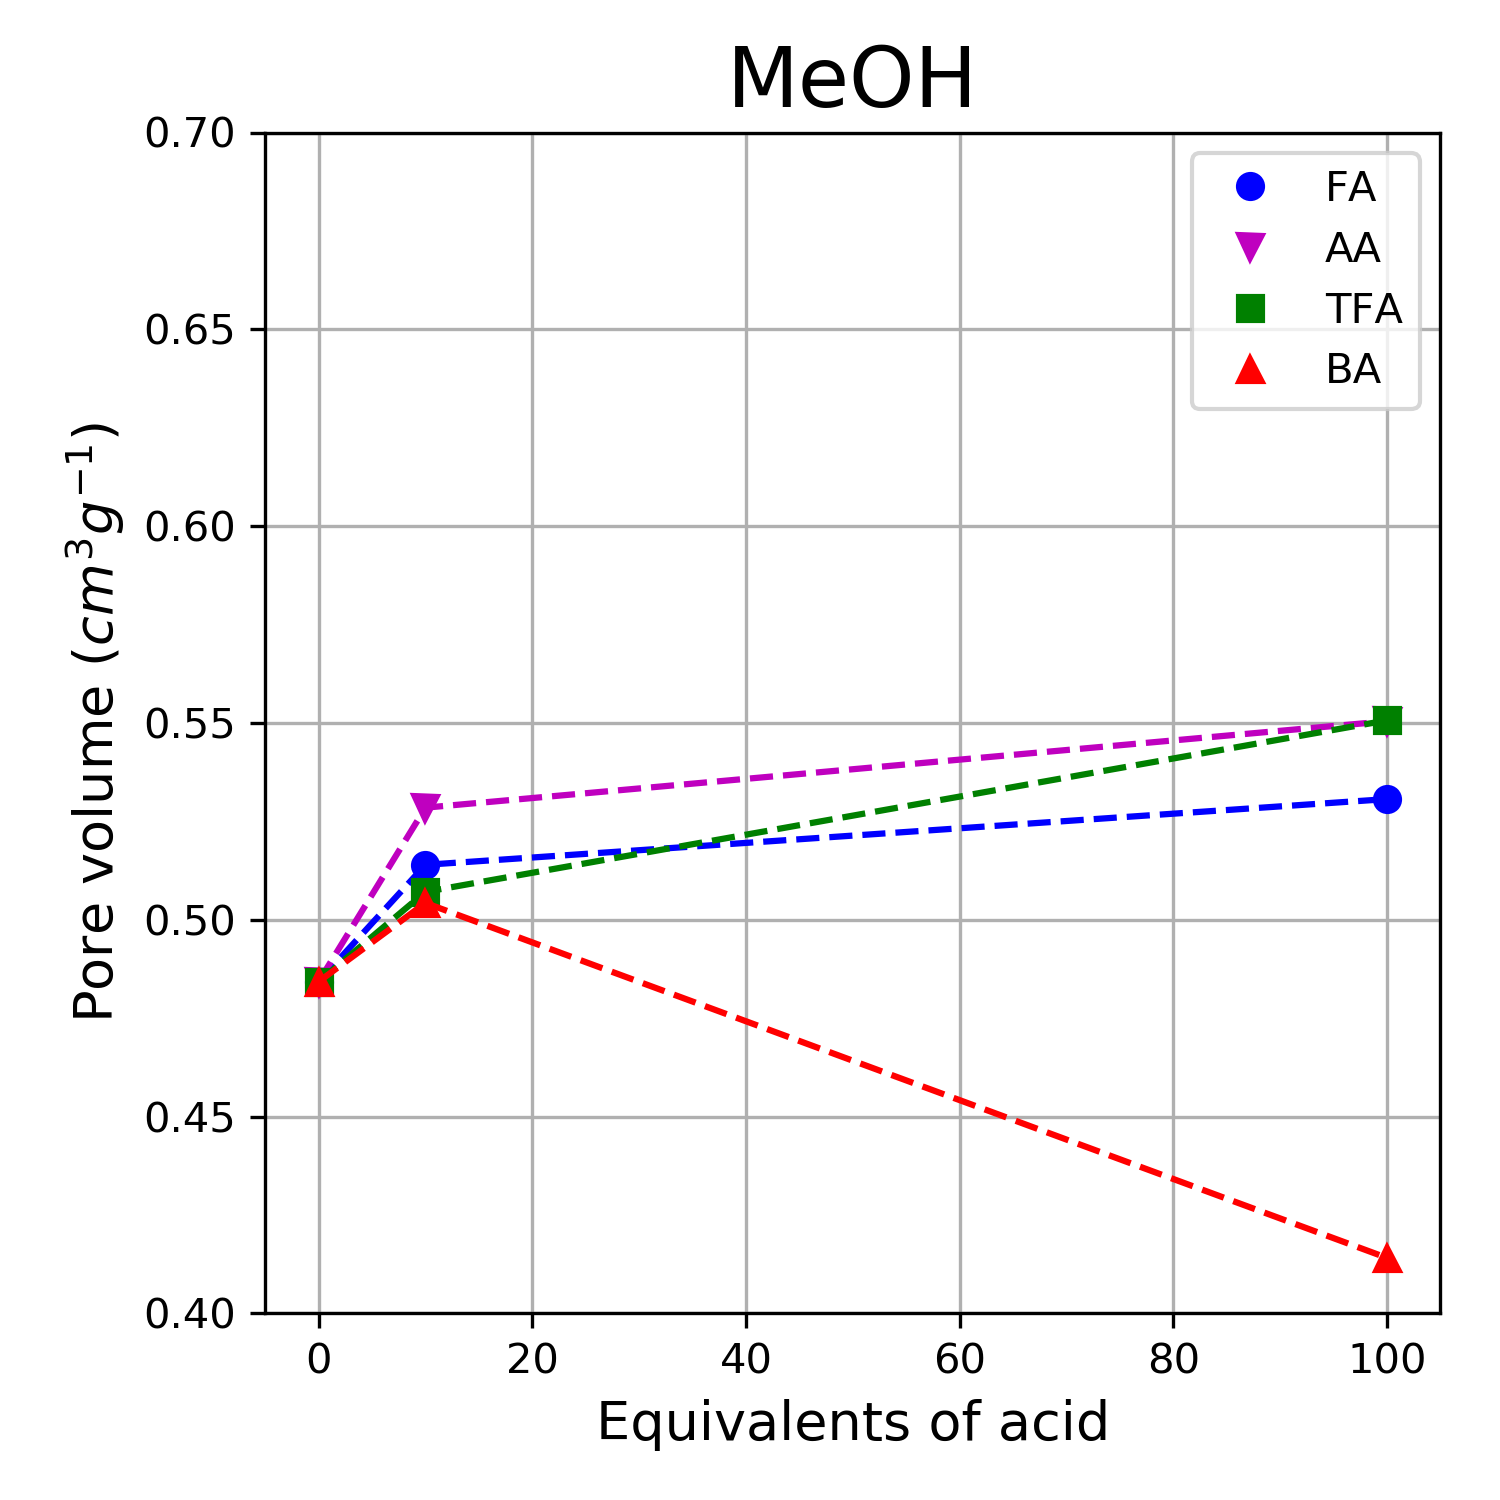
\includegraphics[width=\textwidth]{n2phys/meoh-porevol}%
        \caption{}%
        \label{def:fgr:n2phys-meoh-porevol}
    \end{subfigure}%
    \begin{subfigure}{0.25\linewidth}
        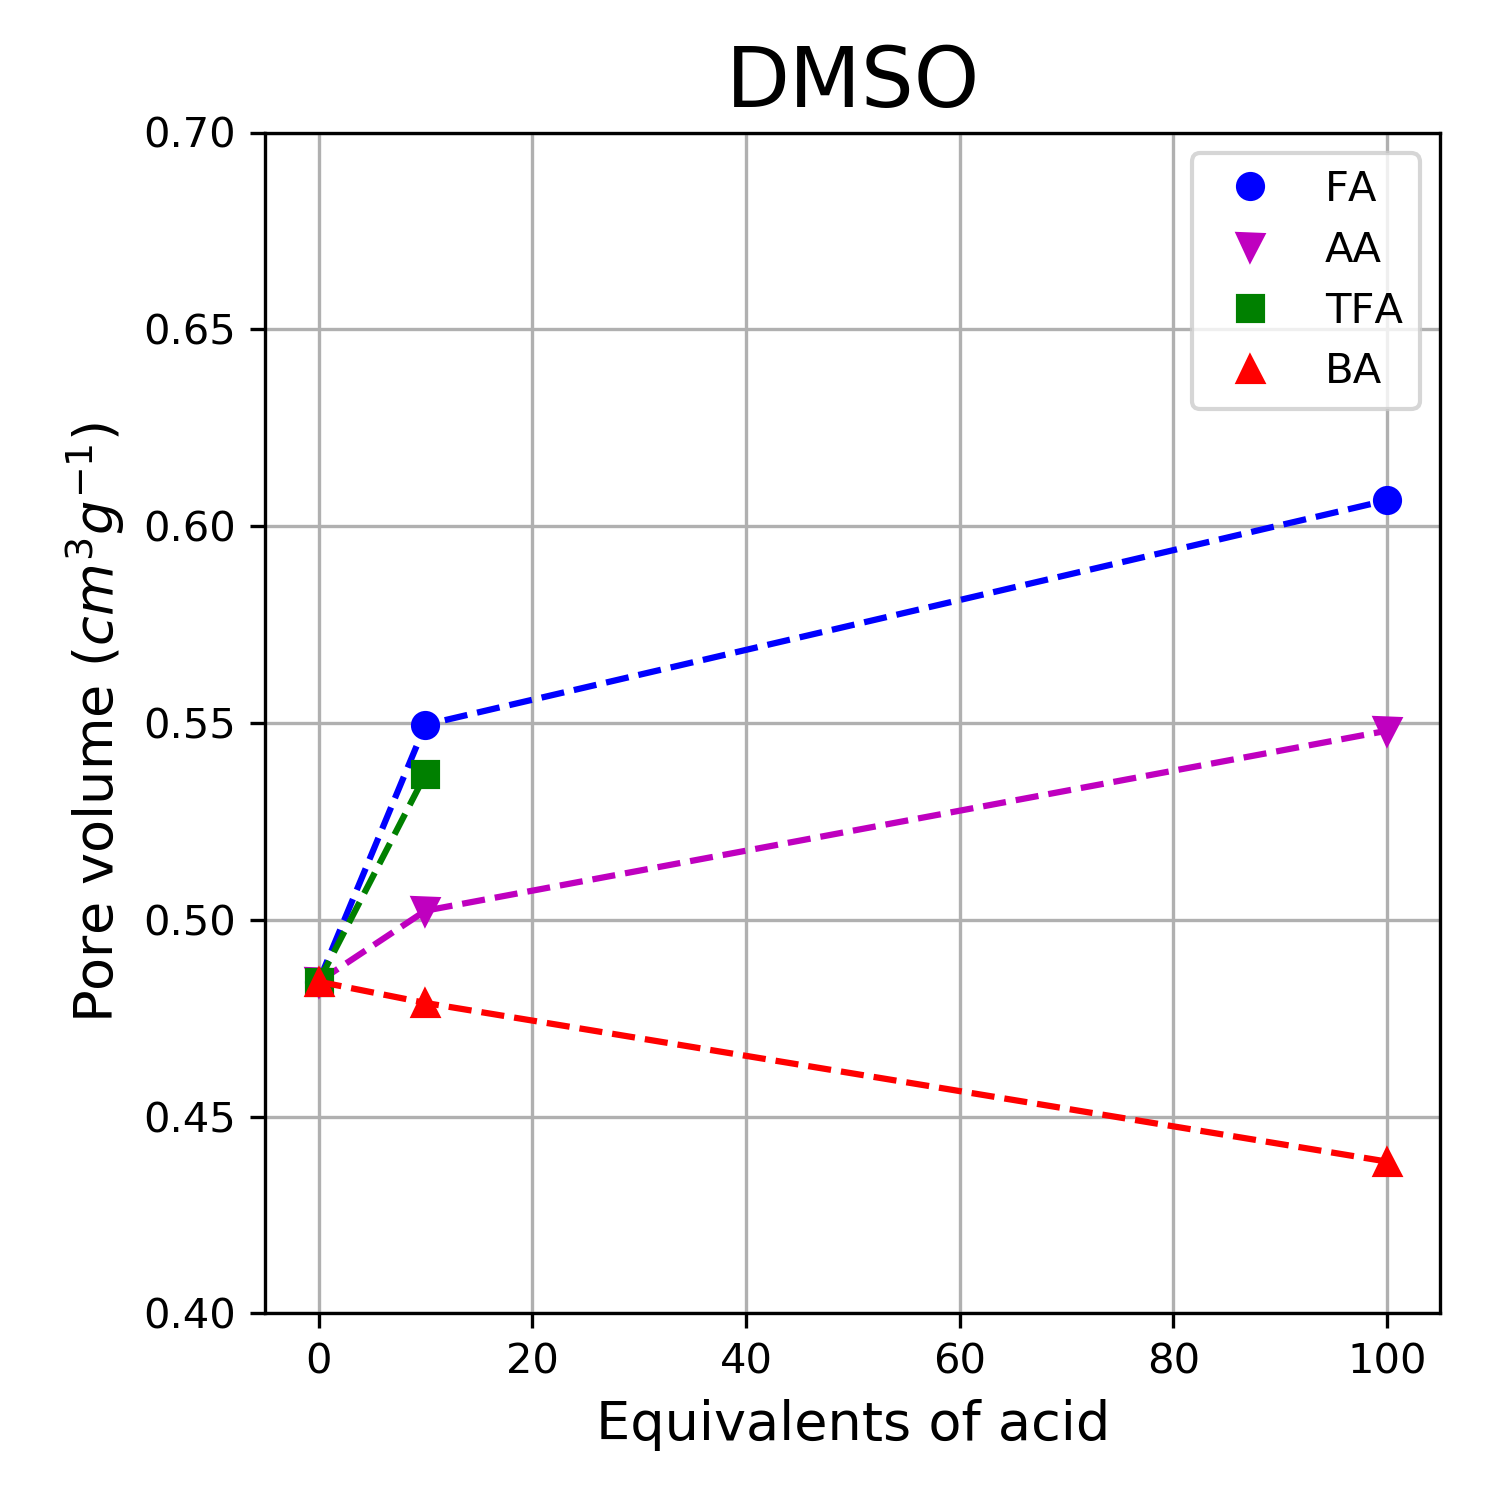
\includegraphics[width=\textwidth]{n2phys/dmso-porevol}%
        \caption{}%
        \label{def:fgr:n2phys-dmso-porevol}
    \end{subfigure}%

    \caption{Characterisation of all samples through predictors
    obtained through processing of the nitrogen physisorption 
    data. The figure shows BET surface area (a-d), the logarithm
    or the initial Henry constant (e-h), the calculated pore volume 
    (i-l) for DMF, \ce{H2O}, MeOH and DMSO leached materials,
    respectively.}%
    \label{def:fgr:nitrogen-predictors}
    
\end{figure}

\todo{check with new results}
The influence of the modulator on the linker-to-node ratio appears to be
constant throughout the solvents used, with an overall trend of 
TFA > FA > AA > BA for generation of defects. The order is similar
to the acidic character of the modulators, except for \todo{table acids?}
benzoic acid which has a lower pKa (4.2) than acetic acid (4.7). 
When examining the influence of the solvent, another trend appears
to emerge, with samples leached in DMSO having the largest propensity
for defect generation, followed by DMF, water and methanol.

In this 
case, the plateau might not be an accurate indication of the number of 
defects since the comparatively large molecule, high boiling point and
similarity to the terephtalate linker in the framework do make its 
removal harder. The nitrogen 